\documentclass[11pt]{article}
\renewcommand{\cite}[2][]{%
\ifx&#2&
    \parentcite{#1}%
\else
    \parencite[#1]{#2}%
\fi
}

\usepackage[utf8]{inputenc}
\usepackage[T1]{fontenc}
\usepackage{lmodern}
\usepackage[left=2.5cm, right=2.5cm, top=2.5cm,  bottom=2.5cm]{geometry}
\usepackage[activate]{microtype}
\usepackage[american]{babel}
\usepackage{verbatim}
\usepackage{graphicx}
\usepackage{svg}
\graphicspath{{svg/}}
\usepackage{xcolor}
\usepackage{csquotes}
\usepackage{amsmath}
\usepackage{amssymb}
\usepackage{nth}
\usepackage{listings}
\usepackage{wrapfig}
\usepackage{float}
\usepackage[inline]{enumitem}
\usepackage{multirow}
\setlist{noitemsep}
\renewcommand{\labelitemi}{$-$}
\usepackage{subfig}
\usepackage{placeins}
\usepackage{footnote}
\usepackage{appendix}
\usepackage[nottoc,numbib]{tocbibind}

\usepackage[
	pdftitle={},
	pdfauthor={},
	pdfcreator={pdflatex, LaTeX with KOMA-Script},
	pdfpagemode=UseOutlines,
	pdfdisplaydoctitle=true,
	pdflang={english}
]{hyperref}

\hypersetup{
	colorlinks=true,
	linkcolor=black,
	citecolor=black,
	filecolor=black,
	menucolor=black,
	urlcolor=black,
	linktocpage=true,
	bookmarksnumbered=true,
	linktoc=all
}

\usepackage[backend=biber,
natbib=true,
maxcitenames=3,
maxbibnames=99,
firstinits=true,
isbn=false,
doi=false,
abbreviate=false,
style=numeric]{biblatex}
\renewbibmacro{in:}{}
\usepackage[linesnumbered,noend,lined,algoruled]{algorithm2e}
\DontPrintSemicolon
\usepackage{tikz}
\usepackage{longtable}

\usepackage[export]{adjustbox}


\bibliography{bibliography} 

\DeclareLanguageMapping{american}{american-apa}

\renewcommand{\cite}{\parencite}
\usepackage{cleveref}

\usepackage{booktabs}
\usepackage{minted}

%\usepackage[compact]{titlesec}
%\titlespacing{\section}{0pt}{*2}{*0}
%\titlespacing{\subsection}{0pt}{*2}{*0}
%\titlespacing{\subsubsection}{0pt}{*2}{*0}
\setlength{\parskip}{10pt}
\setlength{\parindent}{0pt}

\title{
  Fast, scalable WCOJ graph-pattern matching on in-memory graphs in Spark\\
  \vspace{0.6cm}
  \large Master thesis draft iteration 1.2
}
\author{Per Fuchs}
\date{April 2019}

\begin{document}

\maketitle

\abstract{
 Graph pattern matching with their vast number of cyclic foreign-key joins is a new challenge for data processing systems, like Spark, because their intermediary results grow over linear with regards to the inputs and are materialized by the traditionally used binary joins.
 Worst-case optimal join algorithms, WCOJ's, are a natural match to tackle this challenge because they do not materialize the aforementioned large intermediary results.
 We investigate two major open questions regarding WCOJ's.
 First, we develop a WCOJ specialized to graph-pattern matching, namely self-joins on a relationship with two attributes, and compare its performance with a general WCOJ.
 Second, we propose a novel method to distribute WCOJ's. 
 We show in our proposal that current methods to distribute WCOJ's, suitable for Spark, do not scale well to bigger graph pattern (five vertices and more).
 Based on this result we propose to keep the edge relationship cached on all workers but distribute the computation using a logical partitioning.
 Along the line of argumentation in COST~\cite{cost}, we aim to provide a fast WCOJ implementation in Spark which scales well in use of computational resources by trading off scalability in memory usage.
 This is a reasonable trade-off as most graphs today fit in main memory~\cite{snap}. % TODO also cite position paper from Sahihoglus colleague here
 Our thesis provides the first distributed, open-source implementation of a WCOJ in a data processing system widely used in industry, namely Spark.
}

\setlength{\parindent}{0em}
\setlength{\parskip}{0.7em}

\newpage
\tableofcontents
\newpage

\section{Introduction} \label{sec:introduction}





% main idea?
% why is the idea great?


%
% maybe
% snowflake and star join definition?


Newly developed worst-case optimal join (WCOJ) algorithms, e.g. Leapfrog Triejoin, turned conventional thinking about join processing
on its head because these multi-join algorithms have provably lower complexity than classical binary joins,
i.e. join algorithms that join just two tables at-a-time.
In the areas of data warehousing and OLAP, this finding does not have much impact, though,
since the join patterns most commonly encountered are primary-foreign-key joins,
which normally take the form of a tree or snowflake and contain no cycles.
The computational complexity of FK-PK joins is by definition linear in size of the inputs.
In these "conventional" cases, binary joins, e.g. hash joins, work fine.

However, analytical graph queries often use foreign-foreign-key joins, which can grow over linearly in the size of their inputs,
and often contain cycles.
For these use-cases, worst-case optimal join algorithms excel because matching a pattern consisting of multiple joins causes
binary joins to generate a rapidly increasing set of intermediate results, e.g. navigating a social graph with an out-degree in the
hundreds, of which many matches are useless and get eliminated by later joins, e.g. the join closing the cycle.
These kinds of join patterns are frequently found during graph analysis,
e.g. for graph clustering on social network graphs for customer relationship management or recommendation systems
and fraud detection in the financial sector~\cite{fraud-detection,twitter-diamond}.
Worst-case optimal join algorithms avoid large result materialization and hence promise to be orders of magnitude faster than binary joins.
Therefore, we believe that worst-case optimal join algorithms could be a useful addition to (analytical) graph database systems.

% work example for a bit longer
We continue with a short example for a cyclic query and compare how this query is evaluated traditionally and with the new WCOJ's in place.
The simplest example of a cyclical join query enumerates all triangles in a graph.
This can be formulated as the following datalog query
\begin{equation}
    \textit{triangle(a, b, c) $\leftarrow$ R(a, b), S(b, c), T(c, a)} \label{eqn:triangle}
\end{equation} 
 where \textit{R} = \textit{S} = \textit{T} are aliases for the edge relationship.
Traditionally, this would be processed by using multiple binary joins:
\begin{equation}
    R \bowtie S \bowtie T
\end{equation}
% TODO show all join plans
% TODO after executing how many joins?

The join above can be solved in 3 different orders: $ (R \bowtie S) \bowtie T$, $ (R \bowtie T) \bowtie S$ and
$ R \bowtie (T \bowtie S)$.
Independent of the chosen order, database instances exist where the intermediary result size is in $\mathcal{O}(N^2)$ with
\textit{N}= |\textit{R}| = |\textit{S}| = |\textit{T}|.
% TODO put this assumption up and back it by the statement that \textit{R}, \textit{S} and \textit{T} are actually all the same table (edge table).
However, it is provable that output of this query is guaranteed to be in $\mathcal{O}(n^{3/2})$~\cite{agm,skew-strikes-back}
for any database instance.
Hence, binary joins materialize huge intermediary results after processing parts of the query,
which are much bigger than the final result.

The described problem has been shown to be a fundamental issue with traditional binary join plans~\cite{agm,skew-strikes-back}.
We call these plans also \textit{join-at-a-time} approach because they process whole joins at the time.

Fortunately, worst-case optimal join algorithms can materialize cyclic joins with memory usage linear to their output size
by solving the join \textit{variable-at-a-time} which avoids materializing big intermediary results~\cite{leapfrog,nprr}.

In a variable-at-a-time the algorithm finds a binding for the first variable $a$, then one for $b$ and
finally one for $c$.
After this they emit the tuple as part of the output.
Then they find further bindings via backtracking until they enumerated the whole join when all bindings for $a$ have been explored.

A simple example gives an idea why a variable-at-a-time approach is beneficial for cyclic queries.
In \cref{fig:edge-rel-example}, we see an edge relationship.
It is repeated three times labelled with different attributes to ease the understanding of the following explanation;
however, in a systems implementation only one table exist and is used by all joins as input.
% TODO table

A binary join plan which joins $R$ and $S$ via $b$ first produces $16 + 3$ intermediary results;
4 times 4 results for $b = 2$ and one for 6, 11, 12 each.
The next join reduces these 16 results to the three triangle instances; all permutations of the set \{6, 11, 12\}.

A variable-at-a-time approach finds 4 bindings for $a$, namely  $2, 6, 11, 12$;
the intersections of both columns labelled $a$.
Once we fixed a binding for $a$, we find one possible binding for $b$ each;
except the binding $a = 2$ for which we cannot find a matching $b$ value.
Finally, we find all three instances of the triangle by completing the three $a, b$ bindings with
the a $c$ binding.
Apparently we are able to drastically reduce the workload by formulating the join as a problem of
finding variable bindings using information from all parts of the join, instead of, using only one constraint at the time
and building it join-by-join.

We do not claim that the example above illustrates the generality of why binary join plans are provably worse than
\textsc{WCOJ}'s.
Clearly, the example does not show an intermediary result of $N^2$ as $N = 13$ and the intermediary result has the size of 16.
% TODO verify below
However, we note that even in such a simple example all possible binary join orders produce an intermediary result of size 16.
While all possible variable orderings for a variable-at-a-time approaches eliminate the skewed value (2) after finding no binding
for the second variable.
A more general but less concrete and not graph specific example is explained in~\cite{skew-strikes-back}.

% TODO extend.
In practice, these algorithms have been shown to be highly beneficial for cyclic queries in analytical graph workloads in an optimized,
single machine system~\cite{leapfrog,olddog}
and later in distributed shared-nothing settings~\cite{myria-detailed,ammar2018distributed}
- we describe these systems in more detail in~\cref{sec:related-work}.

% definition of graph pattern matching
Graph pattern matching is the problem of finding all instances of a specific subgraph in a graph.
The subgraph to find is described as pattern or query.
In this thesis, we use datalog queries to define subgraph queries.

For example, \cref{eqn:triangle} shows the datalog query describing a triangle.
Here we join three atoms $S, R$ and $T$ with two attributes each $a, b$, $b, c$ and $a, c$ respectively.
The task of enumerating all triangles within the three atoms can be also be described as finding all possible
bindings for the join variables $a, b$ and $c$ within them.

The translation from datalog queries to graph patterns is straightforward.
An attribute or a variable refers to a vertice in a graph and an atom to an edge.
A depiction of the subgraph pattern described by~\cref{eqn:triangle} is shown in~\cref{fig:pattern-triangle}.

In relational terms a graph pattern matching query is an n-ary, conjunctive, self-equi-join on the edge relationship of the graph.
In this thesis, all join queries discussed belong to this sub category of possible join queries.
Other join queries can be useful to describe more complex graph patters, e.g. disjuntion for two edge of which only one needs to
exist or negation to exclude instances that have to many connections.
Some techniques used in this work can be extended to cover these cases, we mention related literature but do not focus
our efforts on these extensions.

% example queries the three from my presentation
% TODO add use cases from Graphflow paper three references, three use cases.
Graph pattern matching is fundamental to analytical graph analysis workloads~\cite{see longbin and semih and presentation}.
We show two graph patterns which are used in practice below and explain the use-cases.

\Cref{fig:pattern-diamond} shows the diamond query which is used by Twitter to recommend their users new people to follow.
The idea is that if a user $a$ is following multiple accounts $c_1, \dots, c_k$ who all follow a person $b$ then it is likely that
$b$ would be interesting to follow for $a$ as well.
In the figure, we see the diamond query for $k = 2$.
This is the diamond query as discussed in most papers in academia~\cite{oldog,myria-detailed,mhedhbi2019}, although,
Twitter uses $k = 3$ in production~\cite{twitter-diamond}.

Our second concrete use-case example, is the n-cycle.
As explained in~\cref{fraud-detection}, cycles can be used to detect bank fraud.
A typical bank-fraud often involves so called \textit{fraud-rings}.
These are two or more people who combine their legitimate contact information in new ways to craft multiple false identities.
For example, two people share real phone numbers and addresses to craft four fake identities (all combinations possible with two pieces
of information).
They open accounts under wrong names with real contact information, use these accounts normally to build trust with the bank and
build up bigger credit lines.
At a certain data the use all credit lines to the maximum and disappear.
The phone numbers are dropped and the actual people living at the addresses deny ever knowing the identities that opened the accounts.

This scheme can be detected using graph pattern matching.
Let us assume, we have a graph database in which customers of the bank, their addresses and phone numbers are all vertices and the
relationship of an address or phone number belonging to a customer are edges.
Then, the case described above forms an 8-cycle of 4 persons (fake identities) connected by the shared use of phone numbers and
addresses.

% spark and graphs
Due to its generality, widespread acceptance in the industry, the ability to use cloud hardware and its fault tolerance by design,
it is an attractive target for big graph processing.
For example, GraphFrames~\cite{graphframe}, GraphX~\cite{graphx} (a Pregel~\cite{pregel} implementation) or graph query languages
as \mbox{G-CORE}~\cite{gcore} and \mbox{openCypher} with their `Cyper for Apache Spark'~\cite{caps} all aim to ease graph processing on
Spark.
The last two technologies translate their graph specific operations to the relational interface of Spark (SparkSQL)
to profit from Spark's relational query optimizer Catalyst~\cite{spark-sql}.
Hence, we believe that the WCOJ's, with their efficiency for analytical graph queries, are a valuable addition to Spark's
built-in join algorithms in general and these graph-on-spark systems in particular.

% research questions
We identify two challenging, novel directions for our research.
First, all of the systems cited above focus on queries widely used in graph pattern matching, e.g. clique finding or path queries.
As explained above, graph pattern matching uses only self-joins on a single relationship with two attributes;
namely the edge relationship of the graph.
However, all systems use worst-case optimal joins developed for general n-ary joins.
This raises the question if and how \textsc{WCOJ}'s can be specialized for graph pattern matching.

Second, while the communication costs for worst-case optimal joins in MapReduce like systems\footnote{
An excellent definition of the term MapReduce like systems is given in~\cite{shares}}
is well-understood~\cite{shares,shares-skew,shares-proof,shares-skew-proof},
their scalability has not been studied in depth.
Given that the only integration in a MapReduce like system exhibits a speedup of 8 on 64 nodes over two workers(an efficiency of 0.125)
~\cite{myria-detailed},
we find that designing a scalable, distributed \textsc{WCOJ} for a MapReduce like system is an unsolved challenge.
It is time to investigate how these algorithms scale in the probably most widely used, general-purpose big data processing engine: Spark.
To the best of our knowledge, this is also the first time a worst-case optimal join is integrated with an industrial-strength cluster
computing model.
We detail our research questions below.
% TODO one sentence about CSR?
\begin{enumerate}
    \item Can we gain performance in \textsc{WCOJ}’s by specializing them to graph pattern matching?
    \begin{enumerate}
        \item How much performance can we gain by using compressed sparse row representations to back the iterators of \textsc{WCOJ}?
        \item Can we exploit the low average out degree of most real-world graphs for the intersections build in a Leapfrog Triejoin?
    \end{enumerate}
    \item How well do \textsc{WCOJ}’s scale in Spark when used for graph pattern matching?
    \begin{enumerate}
        \item How well does Shares scale as a logical partitioning scheme?
        \item How to integrate scalable work-stealing into Spark to counter tuple replication and skew?
    \end{enumerate}
\end{enumerate}


Towards answering our research questions, we make the following contributions.

\begin{enumerate}
    \item We integrate a sequential, general worst-case optimal join, the Leapfrog Triejoin.
      This implementation serves as baseline for our \textsc{WCOJ} optimized to graph pattern matching.
    \item We design and implement \textit{GraphWCOJ} which is a worst-case optimal join specialized to graph pattern matching.
       It is backed by a compressed sparse row representation of the graph which reduces its memory footprint and speeds up execution
       by TODO over a normal \textsc{LFTJ} because it acts as an index. % NUMBER
       Furthermore, we exploit the typical low out degree of most graphs to by specializing the \textsc{LFTJ} for small intersections,
       gaining further TODO x of execution time. % NUMBER
    \item We analyse how many tuples Shares replicates for typical graph pattern matching queries.
      From this analysis and the fact that Shares is an optimal partitioning scheme, we follow that we should replicate the graph
      on all workers for parallelization.
    \item Based on a replicated edge relationship, we design \textit{logical} Shares.
      This is a Shares partitioning which is integrated direclty into the \textsc{WCOJ}.
      We measure a speedup of TODO on 48 workers for some queries and the aforementioned speedup of Myria by TODO.
      The results show that Shares is good in dealing with skew but requires to much replicated work to scale well.
    \item Therefore, we abandon static \textit{logical} partitioning and apply work-stealing.
       We show that workstealing can scale linear on some input queries and beats \textit{logical} Shares for
       all levels for 3-cliques and 5-cliques on three different datasets.
    \item We run experiments on TODO datasets, TODO queries, for up to 96 workers in Spark's local mode using Spark's build in hash join,
       a general Leapfrog Triejoin and our specialize GraphWCOJ.
\end{enumerate}

% TODO limitations
% Only local mode



% TODO results


% structure

% Also introduce cached edge table, ref related work for why communication does not work
% and goals for explanation of why we think caching is helpful
% use mcsherry, other guy here?  --> read them

% These academic systems are not very usable nor used, nor is LogicBlox on the market as a database system.
% For all practical senses and purposes, there are no %systems available that implement WCOJs. Apache Spark is currently the most popular
% analytical data processing system. It does not implement WCOJs yet and has %multiple popular graph processing APIs or subsystems, among
% which GraphFrames, CAPS (neo4j's Cypher on Apache Spark) and the recent LDBC effort to implement the G-%CORE query language on Apache
% Spark. All of these APIs could potentially benefit greatly from a WCOJ algorithm.
% TODO include, just ask.

%Spark offers a well optimized Relational interface [SparkSQL] [Catalsyst]
%Relational interfaces rely on JOINS which have different characteristics different for graphs than for traditional star or snowflake schemes.
 % - they are cyclic for important graph algorithms (cluster, ?subgraphing?)
  %  - large intermediary results which make the queries really expensive for the CPU as well as the in memory
   %   - work is done for nothing because most of the intermediary results are filtered out later
 % - they are highly selective (paths starting from a specific node)
  %  - allowing to safe work when all "filters" are applied simultaneously
  %  - allowing for big jumps on sorted keys with a seek operation, naturally, applied by LFTJ
% - therefore, they are a prime area of application for a new class of join algorithms with worst-case guarantees, which guarantee that no big intermediary results build up
 %because the evaluate multiple joins as once only materializing results that fulfil all join filters.
% - Furthermore, they are naturally suited for highly selective queries because of using an O(log(N)) seek a method to jump over "uninteresting" parts of a sorted result.  

\section{Background}\label{sec:background}

TODO introduction
\subsection{Spark}\label{subsec:spark}
Spark is the probably most widely used and industry accepted cluster computing model.
It improves over former computing models, e.g. MapReduce~\cite{mapreduce}, Hadoop~\cite{hadoop} or Haloop~\cite{haloop},
by allowing to cache results in memory between multiple queries, using so-called resilient
distributed datasets~\cite{rdd}; often abbreviated to RDD.

This section introduces Spark and is organized in four subsections.
\Cref{subsubsec:resilient-distributed-datasets} describes the core data structure of Spark the RDD's.
In~\cref{subsubsec:spark-architecture} we explain the different components and processes in a Spark cluster.
The query optimizer of Spark, Catalyst, is the component of Spark we integrate our \textsc{WCOJ} with; it's structure is explained
in~\cref{subsubsec:catalyst}.
Finally, in~\cref{subsubsec:broadcast-variables} we highlight important details about \textit{Broadcast variables} which are used
to implement our parallel worst-case optimal join.

\subsubsection{Resilient distributed datasets} \label{subsubsec:resilient-distributed-datasets}
RDD's form the core of Spark.
However, for this thesis it is not necessary to understand them in great detail.
In the next paragraph, we give a short introduction into the relevant aspects of RDD's.
For the interested reader, a more in depth description is given in the original paper~\cite{rdd}.

Resilient distributed datasets describe a distributed collection of data items of a single type.
In contrast, to other distributed share memory solutions, RDD's do not use fine-grained
operations to manipulate single data items but coarse grained operation that are applied
to all data items, e.g. \textit{map} to apply a function to each data item.
These operations are called transformations.
An RDD is built starting from a persistent data source and multiple transformation to
apply to this datasource.
One can store the transformations applied to the input data source as in directed acyclic graph, the so called \textit{lineage graph}.
This graph fully describes the dataset without materializing it because the transformations are deterministic.
Hence, the dataset can be computed and recomputed on demand, e.g. when the user asks for the count
of all items in the set.
Operations which require that the data in the RDD is actually computed are called \textit{actions}.

RDD's are distributed by organizing their data items into partitions.
The partitioning can be chosen by the user or the Spark query optimizer such that it allows to run transformations on all partitions
in parallel.
For example, one might chose a round robin paritioning to generate splits of equal size when reading data items from disk or one
groups items by hashing a specific key to support parallelizable aggregation on that key per partition.
The process of repartitioning a RDD is called a \textit{shuffle}.
It is a expensive operations because it involves writing and reading the whole RDD to disk.

Describing datasets as RDD's comes with two main benefits.
First, it is resilient because if the dataset of some partitons of it get lost, it is possible to recompute them from persistent storage
using lineage graph information.
Second, it allows Spark to compute RDD's in parallel.

Spark can parallelize the computation of RDD in two ways.
First, by data-parallelism due to the fact that different partitions of a RDD can
be computed in independently from each other.
Second, by task parallelism due to the fact that some parts of the DAG can be computed without dependence of the others.
Indeed, it is possible to compute all parts of an RDD in parallel which are not related in a topological sort of the graph.

\subsubsection{Spark architecture} \label{subsubsec:spark-architecture}
Spark allows the user to run his program on a single machine or on hundreds of machines organized in a cluster.
In this section, we explain the architecture that allows this flexibility.
\Cref{fig:spark-cluster} shows a schematic Spark cluster setup.

\begin{figure}
    \includegraphics[width=\textwidth]{figures/spark-cluster.png}
    \caption{Schematics of a Spark cluster with two workers, each of them with one exectuor and two threads per executor.Source: Apache Spark Documentation, https://spark.apache.org/docs/latest/cluster-overview.html}
\end{figure}

In Spark, each physical machine is called a \textit{worker}.
On each worker, Spark starts one or multiple Spark processes in their own JVM instance; each of them is called \textit{executor}.
Nowadays, many Spark deployments use a single executor per worker\footnote{This is the setup Databricks uses; Databricks is the leading
maintainer of the Spark platform and offers professional deployment to many customers.}
Each executor runs multiple threads (often one per core on its worker) to execute multiple tasks in parallel.
In total, a Spark cluster can run \textit{\# workers} $\times$ \textit{\# executors per worker} $\times$ \textit{\# threads per executor} tasks
in parallel.

Spark uses two kind of processes to execute an application: a \textit{driver program} and multiple \textit{executors}.
When started, the driver program aquires resources from the \textit{cluster manager} to start its executors.
These executors stay alive during the whole Spark application.
Then, the driver program then continues executing the Spark application.
When it encounters parallelizable tasks, it schedules them on the available executors.

All tasks scheduled on the same executor share a cache for in memory data structures like \textit{Broadcast variables} or persisted RDD
partitions.
This is important in the context of this thesis because it means that we cache the input graph once per executor;
which in many Spark deployments is once per worker or physical machine.
This would not be possible if different tasks in the same JVM would not share the same cache.

Spark allows the user to choose its own cluster manager to manage resources in the cluster.
It comes with good integration for Hadoop YARN~\cite{yarn}, Apache Mesos~\cite{mesos} and Kubernetes~\cite{kubernetes}, as well as,
an standalone mode where it provides its own cluster manager functionality.
Finally, one can run Spark in \textit{local mode} on a single machine using multiple processor cores for worker threads.
In local mode, the driver program and a single executor with as many threads as cores to use share a single JVM.
For our experiments, we run Spark purely in local mode.

\subsubsection{Catalyst} \label{subsubsec:catalyst}
Catalyst~\cite{spark-sql} is Spark's query optimizer.
From a given query, e.g. an SQL query or one described using the DataFrame API, it constructs
in multiple stages an executable \textit{physical plan}.
\begin{figure}
    \includegraphics[width=\textwidth]{figures/catalyst-stages.png}
    \caption{
      Input and stages of the Catalyst optimizer.
      Source: Databricks Blog, https://databricks.com/blog/2015/04/13/deep-dive-into-spark-sqls-catalyst-optimizer.html
    }
    \label{fig:catalyst-stages}
\end{figure}
Its inputs and stages are shown in~\cref{fig:catalyst-stages}.
Below we explain these in order.
We use the triangle given by the datalog rule $COUNT(triangle(A, B, C)) \leftarrow R(A, B), S(B, C), T(A, C), A < B < C $ as
a running example.

The input of Catalyst is a query in the form of a DataFrame or SQL string.
From the optimizer builds a \textit{unresolved logical plan}.
This plan can include unresolved attributes, e.g. attribute names which are not matched to a specific
data source yet or which have no known type.
To resolve this attributes Catalyst uses a \textit{Catalog} of possible bindings which describes the
available data sources.
This phase is referred to as \textit{Analysis} and results in a \textit{logical plan}.
The \textit{logical plan} represents \textit{what} should be done for the query but not exactly \textit{how},
e.g. it might contain a Join operator but not a Sort-merge join.

We show the logical plan for the triangle query in~\cref{fig:triangle-logical-plan}.
As we see, the query is represented as an operator tree where the vertices are operations and the edge indicate dataflow from
one operator to another.
The leaves of the tree are three aliases to the edge relationship
Two of these source relationships are the input the join between \textit{R} and \textit{S} via \textit{B}.
The result of this join and the leave relationship \textit{T} are input to the second join.
The tuples produced by this join are filtered to fulfill $A < B < C$.
Finally, at the root of the tree there is an aggregation to count all results and report the sum.

\begin{figure}
    \centering
    \subfloat[Logical plan\label{fig:triangle-logical-plan}]{\includesvg[width=0.4\textwidth]{triangle-logical-plan}}
    \subfloat[Physical Plan\label{fig:triangle-physical-plan}]{\includesvg[width=0.6\textwidth]{triangle-physical-plan}}
    \caption{Logical and physical plan for the triangle count query as generated by Catalyst.}
\end{figure}

The \textit{logical optimization phase} applies batches of rewriting rules until a fixpoint is reached.
A simple example of a logical optimization would be rewriting $2 + 2$ into $4$.
In our example, this phase pushes the three filters before the root into the two joins and even down to the scans of the input
relationships.

From the \textit{optimized logical plan} the optimizer generates one or multiple \textit{physical plans} by
applying so called \textit{Strategies}.
They translate a logical operator in one or multiple physical operators.
\textit{Strategies} are also allowed to return multiple physical plans for a single \textit{logical plan}.
In this case, the optimizer selects the best one according to a \textit{cost model}.

The physical plan for the triangle query is shown in~\cref{fig:triangle-physical-plan}.
The logical join operators from~\cref{fig:triangle-logical-plan} have been translated to broadcast hash joins and are now preceded by a
broadcast exchange operator.
The exchange operator builds a hashtable from its input operator and makes it available as broadcast variable to all executors of
the cluster; we explain broadcast variables in depth in~\cref{subsubsec:broadcast-variables}.
When an executor is tasked to execute the hash join operator, it aquires the broadcasted hashtable and executes a local hash join
of its assigned partitions.
This is a good example of strategy that translates a single logical operator into two physical operators.
The other change to the logical plan is that the count aggregation has been broken up into an partial aggregation directly after the
last join, an exchange reorganizing all partial counts into a single partition and a second aggregation over that partiton to caculate
the total count.

After generating and choosing a physical plan, Catalyst enters the \textit{code generation} phase in which it compiles Java byte code for
some of the physical operators.
This code executes often magnitudes faster than interpreted versions~\cite{spark-sql} of the same operator because
it can be specialized towards this particular query, e.g. if a join operates only on integers, code
generation can prune all code paths dealing with strings.
Indeed, the code generation phase is part of another Spark project called
\textit{Tungsten}~\cite{tungsten-project,tungsten-code-generation}.
In this thesis, we do not build any code generated physical operators.
Hence, we do not treat this topic in depth.
It is enough to know that all freshly generated Java code is wrapped into a single physical operator.
Therefore, it integrates seamlessly with interpreted operators.

Finally, Catalyst arrives at an optimized physical plan which implements the query.
The execution of this plan is called
\textit{structured query execution}~\cite{spark-internals-structured-query-execution}.
It translates the plan into RDD operations implemented by Spark core.
Hence, the result of Catalysts query compilation is an RDD representing the query.
One should note that \textit{structured query execution} does not actually execute the query: the result is an RDD which is a none
materialized representation of the operations necessary to generate the result.
In this thesis, we are not concerned with the internals of RDD's.
We do not need to introduce any new RDD operations or even touch Spark's core functionality.
Thanks to the extensibility of Catalyst, we can integrate worst-case optimal joins by adding one \textit{logical operator}, multiple
\textit{physical operators} and a \textit{Strategy} to translate the \textit{logical operator} in
its physical implementation.

\subsubsection{Broadcast variables} \label{subsubsec:broadcast-variables}
From the programmer point of view, \textit{broadcast variables} are normal readonly variables.
They are initialized once by the driver program and should not be changed after initialization.
Every serializable type can be used for a broadcast variable.
After intitialization they can be accessed by every task.
When they are not cached the task aquires the value of the variable from the driver program or other workers, deserializes it and
adds it to the cache shared by all tasks on the machine.
Spark guarantees that the each broadcast variable is sent only once to each executor and allows it to be spilled to disk if its not
possible to keep the whole value in memory.
Furthermore, `Spark attempts to distribute broadcast variables using efficient broadcast algorithms to reduce communication
costs'~\cite{rdd-programming-guide}; currently Spark uses a BitTorrent-like communication protocol\footnote{See Spark sources: \texttt{org
.apache.spark.broadcast.TorrentBroadcast}}.

\subsection{Worst-case optimal join algorithm}\label{subsec:worst-case-optimal-join-algorithm}
The development of worst-case optimal joins started in 2008 with the discovery that the output size of a relational query is bound by the fractional edge number of its underlying hypergraph~\cite{agm}.
In 2012, Ngo, Porat, Re and Rudra published a join algorithm matching this bound~\cite{nprr}.
In the same year, Veldhuizen proved that the algorithm ``Leapfrog Triejoin'' used in LogicBlox, a database system developed by his company, is also worst-case optimal with regards to the
fractional edge number bound.
Both alorithms have been shown to be instances `Generic Join' in 2013 Ngo et al.~\cite{skew-strikes-back}.
Leapfrog Triejoin is the only worst-case join algorithm that has been implemented and benchmarked numerous times in widely different settings, e.g. Oxford course work, published research and a commercial database system~\cite{leapfrog,andreas,olddog,myria,ammar2018distributed,leapfrog-triejoin-schroeder}.

\subsubsection{LeapfrogTriejoin}
% TODO LFTJ chapter

\subsection{Distributed worst-case optimal join in Myria}
In 2014, a Leapfrog Triejoin variant, dubbed ``Tributary Join'', was used as a distributed join algorithm on a shared-nothing architecture called ``Myria''~\cite{myria-detailed}.
They use Tributary Join as a local, serial worst-case optimal join algorithm, combined with the Hypercube shuffle algorithm to partition the data between their machines~\cite{hypercube}.
% TODO sort out hypercube and shares usage
However, it is not obvious how well Hypercube shuffles scales because it replicates many of its input tuples~\cite{myria-detailed}.
The combination of Hypercube shuffles and Tributary Join in Myria does not scale well (speedup of 8 on 64 workers compared to the time it takes on 2 nodes) which, although unlikely to be optimal, is not investigated in great detail; we therefore, explain Hypercube shuffles in detail and show that they tend to replicate all data to all nodes for bigger graph patterns~\cref{ssec:hypercube-shuffle}.
Their approach is directly applicable to Spark.
% TODO add Graphflow paper: variable ordering studied, combination of bin + wcoj in plans, query planning first known approach, parallel
% execution?
% TODO check emptyheaded, it uses WCOJ's

\subsubsection{Shares}
% TODO rename HC Shares
We first explain how the Hypercube shuffle algorithm, \texttt{HC}, partitions data.
After, we provide an analysis of its scaling with regards to graph patterns with an increasing number of vertices.

\texttt{HC} partitions the input relationships for a multi-way join over \textit{w} worker nodes, such that, all tuples, which could be joined, end up on the same worker in a single shuffle round.
Hence, it allows running any multi-way join algorithm locally after one shuffle round.
The output of the join is the union of all local results.
\texttt{HC} realizes this partitioning by logical organizing all workers in a hypercube with one dimension per join variable; we call the number of variables \textit{A} and use $a_i$ to reference a single variable.
Each dimension has a size $p_i$, the $p_i$'s have to be chosen such that the constraint $w \ge \prod_{i}p_i$ is satisfied.  % TODO choosing problem
In other words, each worker can be addressed by its coordinate in the hypercube of the form $\{1..p_1\} \times ... \times \{1..p_A\}$.

With this topology in mind, it is straightforward to find a partitioning for all tuples from all relationships such that tuples that could join are sent to the same node.
We choose a hash function $h_i$ for each join variable which maps its values in the range of \{1..$p_i$\}.
Then each worker determines where to send the tuple it holds by hashing its join variables.
This results in a coordinate in the hypercube which is fixed for all join variables, which occur in the tuple, and unbounded for join variables not bound by the tuple.
Then the tuple is sent to all workers with a matching coordinate.
For example, assume a join with three variables $a_1$, $a_2$ and $a_3$ and tuple \textit{t} that binds $a_1$ and $a_2$ then we get the coordinates $h_{a1}(t_{a1}) \times h_{a2}(t_{a2}) \times \{0..p_{a3}\}$ and send the tuple
to all workers with a coordinate matching the first two attributes and arbitrary third component of the coordinate; the tuple is replicated across $p_{a_3}$ machines.

Next, we analyse the scalability of \texttt{HC} on growing graph patterns - that is, joins over a single relationship, the edge relationship of the graph \textit{E} and with two variables per atom.
In this context, atoms of the join can be seen as the edges of the pattern and variables as vertices.
In the following we consider the join query represented by the Datalog rule $Q(a_1, ..., a_A) = R_1(a_1, a_2), ..., R_k(a_{A-1}, a_A)$, we call $atoms(Q)$ the set of all atoms in $Q$, $p_1(R)$ and $p_2(R)$ the $p_i$ corresponding to the variables of $R$.
We use the method described in~\cite{myria-detailed} to calculate optimal shares allocation $p_1 ... p_A$.

Each worker receives $\sum_{R \in atoms(Q)} |R| / (p_1(R) * p_2(R))$ tuples under the assumption of uniform data distribution and good hash functions.
Our argument is that the tuples of each $R$ are divided onto $p_1(R) * p_2(R)$ workers - the workers that form the hypercube planes of its two variables.

In the special case of graph pattern matching where all atoms of the query are pointing to the same relationship, we can optimize \texttt{HC} shuffle such that a tuple is only sent once to a worker, although it might be assigned to it via multiple atoms.
If we apply this optimization, we can predict the probability with which each tuple is assigned to a worker using the Poisson binomial distribution.
The Poisson binomial distribution $Pr(n, k, u_0, ..., u_n)$ allows us to calculate the likelihood that $k$ out of $n$ independent, binary and differently distributed trials succeed, under the condition that the $i$'th trial succeeds with a probability of $u_i$.
We then use $n = |atoms(Q)|$, $k = 0$ and $u_i=1/(p_1(R_i) * p_2(R_i))$ to calculate the probability that a tuple is not assigned to an arbitrary, fixed worker $w$.
This allows us to predict the number of tuples assigned to each worker by $|E| * (1 - Pr(|atoms(Q)|, 0, u_0, ..., u_{|atoms(Q)|})$.

\Cref{table:workload} shows the expected percentage of tuples from $E$ assigned to each node for graph patterns of different sizes calculated using Poison binomial distribution and optimal shares assignments according to the method used in~\cite{myria-detailed}.
As we can see in this table, the number of tuples assigned to each worker grows over linear in the size of the graph pattern and that doubling the number of workers is inefficient to counter this growth.

The second observation has two reasons.
First, doubling the number of workers does not allow to double the dimensions of the hypercube - a hypercube always needs $p_1 \times ... \times p_A$ workers to be built.
Second, the number of replicated tuples increases with a growing hypercube because each tuple from $R_i$ is replicated to $\prod_{R_j \in atoms(Q)/R_i} p_1(R_j) * p_2(R_j)$; due to the fact that each tuple binds only two out of $A$ variables the tuple is replicated over many dimensions, e.g. let the bounded varibales be $a_p$ and $a_s$ then we get  $|\{0..p_0\} \times ... a_p ... \times ... a_s... \times \{0..p_A\}|$ matching worker coordinates.


%First, a hypercube of size $s$ and $A$ dimensions requires $s^A$ workers.
%Second, the replication increases with $A$ and $s$; we argue that each tuple is replicated to $(s+1)^{A-2}$ workers.
%Each tuple binds two out of $A$ variables, let's assume these are $a_p$ and $a_s$ then we have $|\{0..s\} \times ... a_p ... \times ... a_s... \times \{0..s\}|$ matching worker coordinates\footnote{The argument can be rephrased as the number of all strings of the length $A-2$ over the alphabet $\{0..s\}$}.

\begin{table}[t]
    \centering
    \begin{tabular}{lrr}
        \toprule
        Pattern  & Edges  & workload [64]/[128] \\ \midrule
        Triangle & 3                 & 0.18 / 0.12    \\
        4-clique & 6                 & 0.59 / 0.44    \\
        5-clique & 10                & 0.9  /d 0.82    \\
        House    & 5                 & 0.42 / 0.32    \\
        Diamond  & 8                 & 0.76 / 0.67    \\
        \bottomrule
    \end{tabular}
    \caption{Workload, on 64 and 128 workers, in percentage of tuples of the edge table assigned to each worker, using Poison binominial distribution to estimate the workload and the method from~\cite{myria-detailed} to determine the optimal shares configuration.}
    \label{table:workload}
    % See hc-workload-1.csv computed with a28fc458f4f8959a5af81a65f593ea22dcb8dd44
\end{table}

In light of the numbers presented in \cref{table:workload} and in line \cite{ammar2018distributed}, we conclude that the communication costs for \texttt{HC} converge towards a full broadcast for bigger graph patterns and scaling becomes increasingly inefficient.
Anyhow, \texttt{HC} is proven to be communication cost optimal for general multi-way joins in map-reduce like systems in a single round of shuffling in multiple settings~\cite{beame2013,beame2014,beame2016}.
Therefore, we decide to follow a different direction for distributing WCOJ's which we explain in~\cref{sec:goals}.


\subsection{Analysis of public real-world graph datasets}\label{subsec:graph-analysis}
TODO will include histogram of graph sizes, average outdeegree, maybe clustering coefficient and further interesting metrics, with
regards to the thesis, for (all?) graphs of the SNAP and Labaratory of Web Algorithms dataset collection.

\subsection{Compressed sparse row representation}\label{subsec:csr-background}
Compressed sparse row representation (short CSR) is a well known, low-memory representation for static graphs~\cite{csr,csr-first}.
To ease its explanation, we assume that the graph's vertices are identified by the numbers from 0 to $|V| - 1$.
However, our implementation allows the use of arbitrary vertice identifiers in $\mathcal{N}$ by storing the translation in an additional
array of size \textit{|V|}.

CSR uses two arrays to represent the edge relationship of the graph: one of size \textit{|E|} which is a projection of the edge relationship
onto the \textit{dst} attribute and a second of size \texttt{|V + 1|} which stores indices into the first array.
To find all destinations directly reachable from a source \textit{src $\in$ V}, one accesses the second array at \textit{src} for the
correct index into the first array for a list of destinations.
% TODO maybe example figure?

The CSR format has two beneficial properties in the context of this thesis.
First, it allows locating all destinations for a source vertice by one array lookup;
hence, in constant time.
Second, the representation is only, roughly, half as big than a simple columnar representation.
A uncompressed columnar representation needs $2 \times |E|$ while CSR uses only $|V| + 1 + |E|$, note that for most real-world graph |V|
<< |E| holds (see~\cref{subsec:graph-analysis}).



% Parallelism in Spark
% ====================
%We give examples for both kind of parallelism in the triangle count query
%(\cref{fig:lineage-triangle}).
%Lets assume that the CSV file is partitioned in 10 equal parts and each part is read
%by one out of 10 workers.
%Then the resulting RDD has 10 partitions.
%The following filter can be applied to all 10 partitions in parallel.
%This computation is also task parallel because all three filters can be applied to the
%input set directly after reading it from disk.

%If we go one step further into the example of the triangle query and look at the first
%join, we see limitations to Spark's parallelism.
%Let's assume that we want to use a Hashjoin implementation.
%In this case, we have to build a hash table of either side of the join.
%Hence, the computation of the join needs to wait until this hash table has been build.
%This is clearly not task parallel and it's also not data parallel on the build site
%because we need the data from all partitions to construct a full hash table.
%The result is that we see an exchange operator in the DAG of \cref{fig:triangle-lineage}.
%This operator allows to reorganize the partitions of a RDD.
%In the case of a hash join, it would reorganize items from all partitions into a hash
%table and make copies of this hash table available to the tasks that compute the
%partitions of the join.

%In the last paragraphs, we covered that Spark uses data parallelism arising from the partitioning of the RDD's
%and task parallelism arising from the lineage-graph representation of the RDD's.
%Synchronization happens via exchange operators which allow to reorganize the paritioning of the RDD's.
%In the following, we explain how Spark exploits parallelism in its execution model.

%Spark uses a scheduler to assign \textit{tasks} to \textit{slots}.
%\textit{Tasks} are the smallest unit of work in Spark.
%They are created by dividing the RDD lineage graph into pipelinable \textit{stages}.
%Normally, a stage consists out of all transformations between two exchange operators.
%Each stage consists out of as many tasks as it has partitions.

%The stages of the triangle query are shown in \cref{fig:triangle-lineage}.
%We have four stages.
%Two to build the hash table for our hash join which start with reading the CSV from disk and end with the exchange operator before
%the join.
%The longest stage also reads the CSV from disk, includes the two streaming sites of the hash joins and finally aggregates all
%results per partition for the count.
%It ends with an exchange to aggregate the counts of all partitions; this aggregation is the last out of for \textit{stages}.
%
%These four stages lead to 31 tasks if we assume that each stage starts with reading the CSV into 10 partitions.
%This is because the first 3 stages have 10 tasks each and the last stage accumulating all counts after the last task is only as single
%task of summing up all partitions of its parent.

\section{Worst-case optimal join parallelization}  % TODO header

Based on the fact that Shares is an optimal partitioning scheme for n-ary joins in MapReduce like systems~\cite{shares} and
our analysis that Shares converges to a full broadcast of the graph edges (see \cref{shares-proof}), we decided
to forego physical partitioning of the graph.
We cache the graph in memory such that each Spark task can access the whole graph.
Then, we experiment with multiple \textit{logical} partitioning schemes which ensure that each task processes
only some parts of the graph.

This design allows us to implement a new flavour of the Shares partitioning in which we filter the vertices of the
graph on-the-fly while processing it with our \textit{Graph\textsc{WCOJ}} algorithm.
We describe this contribution in \cref{ssec:shares-logical}.

Furthermore, we consider a work-stealing based partitioning which does not replicate any work and produces less
skew than Shares. % TODO is that always correct.
This comes at the price of implementing work-stealing on Spark.
The design of work-stealing in Spark is described in \cref{ssec:work-stealing}

\subsection{Logical Shares} \label{ssec:shares-logical}
Shares has been developed as a optimal shuffle for n-ary joins on MapReduce like systems.
So, it is used to physical partition the tables participating in the join over all workers of the system.
Then, each worker works only on the tuples it holds in its partition.
This has been implemented in Myria for \textsc{WCOJ}~\cite{myria-detailed} and for Haddoop~\cite{TODO}.
We describe the Shares and Myria in more detail in~\cref{ssec:myria} and assume that the reader is familiar
with this section.

The idea of Shares can also be used for a \textit{logical} partitioning scheme.
Instead, of partitioning the graph before computing the join, we determine if a tuple should be considered by the
join on-the-fly.
We implement and measure this idea for multiple reasons.
First, as a baseline for further partitioning schemes.
We argue that it is a good baseline because it has been proven to be an optimal physical partitioning scheme and
has been used by systems similar to us.
Second, to practically show our point that Shares is not scaling due to the high amount of duplicated work.
Third, to investigate the possibility of combining the Shares algorithm and the \textsc{LFTJ} algorithm in
a way that improves scaling.

% TODO list of points
Variables can be filtered independently from each other, e.g. once a tuple does not match the coordinate for one variable it is out. Hence, I can filter the TrieIterator levels independently from each other - exclude on the first level and then again on the lower level.
Push as deep as possible

Pushing the filter into the binary search does not help. The binarys search consists out of a binary search followed by a linear search - we analyse them in this order. Let’s assume we never search for an element which should not be considered in the first place. Then each none-to-consider element will be touched to find the direction of the search to continue, it does not matter if it’s to consider at all.
If the element is not found by the binary search until the search space becomes small, it is searched by a linear search. If any none-to-consider element is smaller than the key, it has been read before we can know it was not to consider, we are fastest by just continuing. If the any none-to-consider element is bigger, the search ends anyway. It only changes which upper bound it will return. It will be slightly faster to return a to-consider upper bound directly because otherwise the search needs to be started again and again until a to-consider upper bound is found. I should support a filtered upper bound search or filter that out by a special case.
To conclude my day, I have a first, not yet correct version of a logical Shares partitioning scheme. The main problem is that it is damn slow. With filtering the algorithm takes way longer than without. This seems to be mostly caused by my jumping over filtered vertices one-by-one. However, it is also partly caused by the implemenation as decorator, only leading all calls through a nop-decorator already looses 1 second to an none-decorated TrieIterator execution.

Idea: filter for shares after the Leapfrogjoin. Why should that be faster? The Leapfrogjoin is a filter in itself. If its selectivity is much higher than Shares, it would be faster to filter for Shares afterwards. Also, Leapfrogjoin employs binary search to jump over huge sets of vertices, probably we should spent the work of Shares fitlering after this.


Shares configuration computation: on master, same algorithm as in Myria, sometimes quite long TODO number, not optimized,
discussed in great detail in the myria paper, 06.08


\subsection{Work-stealing} \label{ssec:work-stealing}

\section{Graph\textsc{WCOJ}} \label{sec:graphwcoj}
TODO
\subsection{Combining \textsc{LFTJ} with \textsc{CSR}} \label{subsec:graphWCOJ-csr}
For our graph pattern matching specialized Leapfrog Triejoin version we choose \textsc{CSR} (see \cref{subsec:csr-background}) as
backing data structure.
This data structure is typically used for static graphs and we show that it is a great match for \textsc{LFTJ}.
In this section, we shortly describe the implementation of a \textsc{CSR} based \textit{TrieIterator}, point out the differences between
this new version and a column-based \textit{TrieIterator} (as described in~\cref{subsubsec:leapfrog-triejoin}) and conclude with an experiment demonstrating
the power of this optimization.

The implementation of a \textsc{CSR} based \textit{TrieIterator} is straightforward except for one design change: instead of using
the vertice identifier from the graph directly, we use their indices in the \textsc{CSR} representation.
This change is rather minor because it can be contained at any level by using a hash map for translation, e.g. in the
\textit{TrieIterator} itself, in the \textit{LeapfrogTriejoin} or at the end of the query by an additional mapping operation.

In the current system, the translation is performed by the \textsc{LFTJ} implementation to allow easy integration into other projects.
However, it is possible to work on the indices throughout the whole system to safe the translation costs.

We now outline how to implement each of the \textit{TrieIterator} methods, under the assumption that all vertices have outgoing edges.
Then, we drop this assumption and explain the necessary changes.
The creation of the \textsc{CSR} data structure itself is described in~\cref{subsec:spark-integration-graphWCOJ}.

We recall that a CSR uses two arrays to represent the graph edge relationship;
the \textit{AdjacencyLists} array and \textit{Indices} array.
The first one stores all adjacency lists in one direction (outgoing or incoming) as one concatenated array.
The second stores indices into the first array, e.g. the value of 5 at position 1 means that the adjacency list
for the second vertice starts at the 5th position in \textit{AdjacencyLists}.

The vertical component of the \textit{TrieIterator} consists out of the \textit{open} and \textit{up} methods.
Both of them control on which of the two \textsc{CSR} arrays the iterator operates.
For the first level, it uses the \textit{Indices} array and on the second level the \textit{AdjacencyLists} array.

The \textit{open} method does nothing when the first level is opened.
When the second level is opened, it positions the iterator at the first element of the adjacency list.
This position is given by the index in \textit{Indices} where the first level is positioned.

Both methods use only constant time.
This differs from the \textit{open} method of the array based \textit{TrieIterator}.
This method needs to find the number of second-level elements when the second level is opened;
it does so by counting the number of occurrences of the first level key in the first column.
Additionally, both vertical component methods have more bookkeeping overhead for the array-based implementation.

The linear component of the \textit{TrieIterator} is made of the functions: \textit{key}, \textit{atEnd}, \textit{seek} and
\textit{next}.

The \textit{key} and \textit{atEnd} method are both only returning values computed by \textit{next} or \textit{seek}.
They do not differ for the \textsc{CSR} based and array based \textit{TrieIterator}.

The \textit{next} method of the CSR based \textit{TrieIterator} only changes at the first level.
While the array-based method needs to use the \textit{seek} method to find the next higher value because
it needs to jump over all entries of the same value as the current key, the CSR based value can simply increase
the iterator position by one.

The \textit{seek(key)} method exhibits the biggest possible performance improvement on the first level.
For the array-based version, we need to use a binary search to find the \textit{key}.
A CSR allows us to jump to the correct position in constant time because the \textit{key} parameter is the correct
index into the array.

To resolve the assumption of no empty outgoing adjacency lists, we adapt \textit{open}, \textit{next} and \textit{seek} to skip source
positions without outgoing edges.
This is easy to detect because then $Indices[x] = Indices[x + 1]$.
We can skip these cases by simple linear search until we find a valid position.
This solution is sufficient because there are only a few vertices with no outgoing edges in real-world graphs.
Therefore, this linear search does not majorly influence the run time.

The \textit{TrieIterator} implementation based on \textsc{CSR} is much faster than the column based iterator; mainly due to the fact
that the \textit{seek} method on the first level can be implemented in $\mathcal{O}(1)$, instead of $\mathcal{O}(\log n)$.
This optimization has huge potential because these searches are the most costly operations for a column-based
\textit{TrieIterator}~\cite{myria-detailed}.
Note that searches on the second level are fast, due to the fact that most graphs have a low outdegree (see
\cref{subsec:graph-analysis}).

Additionally to this advantage, \textsc{CSR} based \textit{TrieIterator} do less bookkeeping because they support only 2 levels and spent
nearly no time on processing \textit{atEnd} for the second level, while a column based \textit{TrieIterator} needs to calculate the
number of outgoing edges for each source vertice in its \textit{open} method, to allow a fast \textit{atEnd} method.

We conclude that \textsc{CSR} based \textit{TrieIterator}'s are a promising match for \textsc{LFTJ} and graph pattern matching.
The improvements of this optimization can be seen in \cref{fig:wcoj-vs-graphWCOJ}.
It demonstrates an up to 2.6 speedup over a column-based \textsc{LFTJ}. % NUMBER
We also see that the optimization has a stronger impact on queries with more edges and vertices, e.g. \texttt{5-clique}.
For a more thorough evaluation refer to the experiment section \ref{sec:experiments}.

\begin{figure}
    \centering
    \includesvg[width=0.5\textwidth]{svg/wcoj-csr}
    \caption{Run time of \textsc{LFTJ} and GraphWCOJ backed by \textsc{CSR} for multiple queries on \texttt{SNB-sf1}.}
    \label{fig:wcoj-vs-graphWCOJ}
\end{figure}

\subsection{Exploiting low average outdegrees} \label{subsec:graphWCOJ-materalization}
% TODO study in backgrounda

It is well-known that most real-world graphs have a low average outdegree, mostly far below 200.
This leads to the hypothesis that the intersection of multiple adjacency lists is small, e.g. below 10 in many cases.

We can exploit this fact by materializing the intersections in the \textit{LeapfrogJoins} directly
in one go; instead of, generating one value at-the-time in an iterator like fashion as described in the
original paper~\cite{lftj}.
We believe this to be beneficial because it allows us to employ a simpler intersection algorithm which builds
the intersections touching each adjacency list only once, instead of, multiple times with yielding like the original
\textit{LeapfrogJoin} (see~\cref{alg:leapfrogSearch}).

We structure the remainder of this section as follows.
First, we shortly reiterate the most important facts about \textit{LeapfrogJoins} for this chapter.
Second, we analysis the intersection workload in terms of input sizes and result size to confirm our hypothesis
and gain valuable insights to choose the best intersection algorithm.
Third, we explain the algorithm we chose based on the analysis.
Fourth, we point out differences to the original Leapfrog Triejoin.
Finally, we present a short experiment showing the performance gains of this optimization.

\textit{LeapfrogJoins} build the intersection between multiple adjacency lists.
This is done in an iterator-like fashion in their \textit{leapfrog\_search} method by repeatedly finding the upper-bound for the largest
value in the lowest iterator.
This algorithm is asymptotically optimal for the problem of n-way intersections.
However, we believe that it is (1) to complex for small intersections and (2) should generate all values at once instead of one-by-one to
improve performance on real-world adjacency lists.

To determine the best algorithms to build the n-way intersection in the \textit{LeapfrogJoins},
we run some experiments to characterize the workload.
Towards this goal, we log the size of the full intersection, the size of the smallest iterator participating
and the size of the largest intersection between the smallest iterator and any other iterator on 5-clique queries on \texttt{SNB-sf-1}.
\Cref{fig:intersection-workload} depicts these metrics as cumulative histograms.
In the next paragraphs, we point out the most important observations in each of these graphs.

\Cref{fig:intersection-workload-smallest} shows the size distribution of the smallest iterator, as to be expected for a social network
graph, the outdegree is between 1 and 200.
We do not see the long-tail distribution typical for power-law graphs because we choose the smallest iterator out of 5 and even
though there are vertices with a much higher outdegree, the chance of encountering 5 of these in a single intersection is small.
We note that in 80\% of all cases the smallest iterator has a size lower than 80 and above that the distribution slowly increases to 100\%
% NUMBER

\Cref{fig:intersection-workload-smallest-biggest} illustrates the size distribution of intersecting the smallest iterator with any other
iterator, such that the intersection is maximal.
We choose this specific metric to motivate one of our design choices later on.
As for the smallest iterator, some of these intersections are as big as ~200 but most of them are much smaller.
However, unlike for the smallest iterator metric, 80\% of the intersections contain less than 21  elements and the frequency increases to
100\% in a steep curve.

This last observation is even stronger for the size of the total intersection (\cref{fig:intersection-workload-total}):
the size is less than 5 in 80\% of all intersections and increases similarly steep to 100\%.
The maximum is lower than 200.

These observations confirm our hypothesis that the size of the intersections is small (below 5) and do not show the same long-tail
distribution as the whole social network graph.
Hence, we can materialize them without running at risk of building big intermediary results.

Furthermore, the experiment shows that optimizing by taking iterator sizes into account is worthwhile but only for the smallest iterator
because
once we start with the smallest iterator the further intersections are small (below 21) in the vast majority of all instances.


\begin{figure}[H]
    \centering
    \subfloat[Smallest iterator\label{fig:intersection-workload-smallest}]{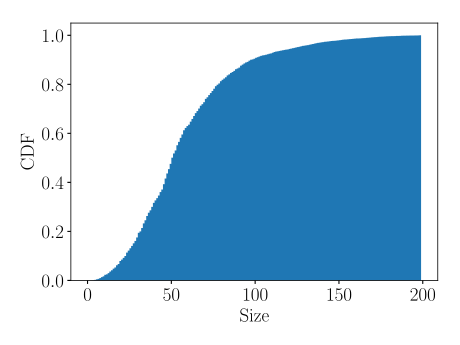
\includegraphics[width=0.3\textwidth]{intersections/smallest.png}}
    \hfill
    \subfloat[Largest intersection including smallest iterator\label{fig:intersection-workload-smallest-biggest}]{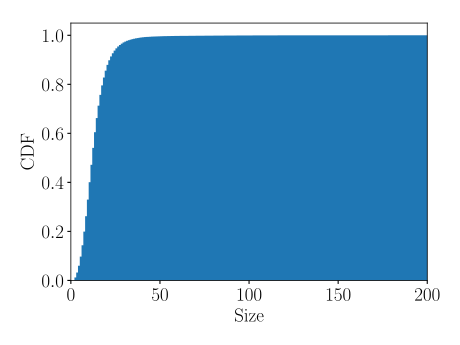
\includegraphics[width=0.3\textwidth]{intersections/smallest-biggest.png}}
    \hfill
    \subfloat[Total intersection\label{fig:intersection-workload-total}]{\includegraphics[width=0.3\textwidth]{intersections/total.png}}
    \caption{Cumulative histograms of total intersection sizes, largest intersection with the smallest iterator and any other, and size of the
    smallest iterator participating in \texttt{5-clique} on \texttt{SNB-sf-1}.}
    \label{fig:intersection-workload}
\end{figure}

In the coming paragraphs, we detail how to build the n-way intersection of multiple adjacency list
such that we gain performance by better use of data-locality than original the \textit{LeapfrogJoin}.
We choose to use pairwise intersections over multi-way intersection algorithms for their simpler memory access patterns;
they touch only two lists at-a-time instead of all lists interchangeably.

From our analysis, we conclude that the final intersection size is strongly dependent on the
smallest iterator and that the intersection of the smallest iterator with any other iterator is
close to the final size.
These insights translate into two design decisions.

First, we start with the smallest iterator\footnote{We take advantage of the fact that CSR allows us
to determine the size of iterators cheaply (see~\cref{subsec:csr-background})}.
However, we do not take the sizes of any other iterators into account because the effort for
sorting the iterators by size would not pay off.

Second, we use two different tactics to build the pairwise intersections.
The first intersection between two iterators is built \textit{in-tandem},  where we seek
the upper bound of the higher value in the smaller iterator.

After this first intersection, the intermediary result is quite small.
Therefore, we use the simpler scheme of linearly iterating the intermediary and probing
the iterator by binary search with fall-back to linear search.

Finally, we point out a few exceptional cases and pitfalls for implementors:
\begin{itemize}
    \item If all iterators of the \textit{LeapfrogJoin} are on their first level, the intersection is near |V|. In this case, we fall back
    to the original
    \textit{LeapfrogJoin}.
    \item We use an array to materialize the intersections because Scala collections are slow.
    Instead of deleting elements, we replace them with a special value.
    \item Allocating a new array for every \textit{LeapfrogJoin} initialization is costly.
    We estimate the size of the intersection by the size of the smallest iterator and reuse the array whenever possible. We use a sentry element to mark the end of the array.
\end{itemize}

\Cref{fig:mat-nomat-short} shows that the new algorithm performance slightly better than
the original on fast-running queries on the \texttt{SNB-sf1} dataset.
We believe that this has three possible reasons.

\begin{figure}[H]
    \centering
    \includesvg[width=0.5\textwidth]{svg/mat-nomat-short}
    \caption{Runtimes of \texttt{GraphWCOJ} with and without \textit{LeapfrogJoin} materialization
    enabled for different queries on \texttt{SNB-sf1}.}
    \label{fig:mat-nomat-short}
\end{figure}

First, due to better cache usage.
Most of the searches in the adjacency lists are linear searches;
our binary search falls back to a linear search if the remaining list is small.
Materializing the intersections means repeating linear searches for increasing elements on the same
two arrays until they are fully processed.
While the original algorithm repeats linear searches overall adjacency lists, interrupted from filtering
against first level iterators and does so only until one value is found;
it then has to return to the same lists for the next elements.

Second, the \textit{LeapfrogJoin} generates a single value, then yields control to other parts
of the \textit{LeapfrogTriejoin} algorithm and later touches the same adjacency lists again to generate the next value.
Our approach touches the adjacency lists exactly once per \textit{LeapfrogJoin} initialization and
condenses the intersection into a much smaller array.
This array is more likely to stay cached while the other parts of the \textit{LeapfrogTriejoin} do their work.

Third, by starting with the smallest adjacency list of the intersection we get less \textit{seek}
calls to iterators over bigger adjacency lists.

We show the results of more experiments in \cref{subsec:lftj-vs-graphWCOJ}.
\section{Implementation}\label{sec:implementation}

\subsection{General sequential version (\textit{seq})}\label{subsec:general-sequential-version}
We implement the Leapfrog Triejoin~\cite{leapfrog} as our general sequential version of a WCOJ.
However, instead of using B-Trees as a backing data structure, we use sorted arrays and a binary search
to for its backing, which has been described in~\cite{myria-detailed} and is called Tributary join in their paper.
Our Leapfrog Triejoin is implemented in three components, which we explain in this order below: \textit{LeapfrogJoin}, \textit{ArrayTrieIterable} and
\textit{LeapfrogTriejoin}.

The Leapfrog join is a variant of the sort-merge join for unary relationships, original described in~\cite{leapfrog1,leapfrog2}. % TODO see LFTJ paper 4 and 7
To join $k$ unary relations $A_1(x)$, $A_2(x)$, \dots, $A_k(x)$ it takes one iterator per input relations and offers an iterator
interface that yields the intersection of all relations.
It requires that it's input iterators offer a \textit{key} method in $\mathcal{O}(1)$, a \textit{next} method and
a \textit{least\_upper\_bound(key: Int)} both in $\mathcal{O} (\log n)$ ($n$ defined as the size of the input relationship).
\textit{least\_upper\_bound} moves the iterator to the first position of the sought \textit{key} or the first position of the
next higher value.
An idiotmatic implementation of a Leapfrog join is shown in~\cref{lst:leapfrog-join}, for the optimized implementation see
\texttt{leapfrogTriejoin.LeapfrogJoin} in our repository.  % CODEREF

\begin{listing}[H]
    \inputminted{scala}{code/LeapfrogJoin.scala}
    \caption{Leapfrog join.}
    \label{lst:leapfrog-join}
\end{listing}

To support j-arity relations, $A(a_1, a_2, \dots, a_j)$ we add two methods to the iterator interface that represents the input
relationships: \textit{up} and \textit{down} both are required to work in $\mathcal{O} \log n$.
We call this new iterator \textit{Trieiteraor} because it represents the relationship as a trie, see~\cref{fig:trie-example}.

% TODO Trieiterator not in textit
The implementation of a \textit{Trieiterator} backed by a columnwise representation of the relation using one array
per column is straight forward, we outline the basic ideas next and refer to the interested reader to
\texttt{leapfrogTriejoin.ArrayTrieIterable.TrieIteratorImpl} in our repository for further details.  % CODEREF
It helps to think about the \textit{Trieiterator} as consisting out of a linear component, containing the functions
\textit{key}, \textit{next} and \textit{seek}, and horizontal component, made off the functions \textit{up} and \textit{down},
to move the linear component from one trie level to another.
First, we explain the horizontal component.
They keep track of the current \textit{level} of the \textit{Trieiterator} and the \textit{startPosition} and \textit{endPosition}
for in the columns,
e.g. in~\cref{fig:trie-example} when the current \textit{level} is 1 (or x) and the key equals 4 the \textit{startPosition} is 2 and
the \textit{endPosition} is 5 because the value 4 occurs 3 times.
With these bookkeeping variables, updated by \textit{up} and \textit{down}, one can implement the linear part by
a binary search over the current column (given by \textit{level}) which is limited to \textit{startPosition} and \textit{endPosition}.

\begin{figure}
    \centering
    \includesvg[height=5cm]{trie}
    \caption{A 3-ary relationship as table (left) and trie (right), to position the iterator at the tuple (1, 1, 5) one
    calls \textit{down} twice, \textit{key} returns now 5, after a call to \textit{next}, \textit{key} returns 6 and \textit{up}
    would lead to \textit{key} returning 1.}
    \label{fig:trie-example}
\end{figure}

The Leapfrog Triejoin combines \textit{Trieiterators} and Leapfrog joins to join $k$ relationships of arbitrary arity.
Its input is one \textit{Trieiterator} per relationship, from this it builds one Leapfrog join per attribute which
receives references to all \textit{Trieiterators} of relationships containing this attribute, e.g. for the triangle query
\textit{R(a, b), S(b, c), T(a, c)} the Leapfrog Triejoin receives three Trieiterators, for \textit{R}, \textit{S} and \textit{T},
and builds three Leapfrog joins, for $a$, $b$, $c$, which receive references to two TrieIterators each.
To generate the join result the Leapfrog Triejoin operates the horizontal components of the Trieiterators directly and
uses the Leapfrog joins to operate the linear component.

% TODO can I reference lines?
We show an idiomatic implementation in~\cref{lst:leapfrog-triejoin}, a performance oriented implementation can be found in our
repository in \texttt{leapfrogTriejoin.LeapfrogTriejoin}.
The listings contains two important functions: the initialization function from line TODO to line TODO % LINE
and the \textit{moveToNextTuple} function at line TODO. % LINE
We go through these functions in order.
The initializer gets two arguments: a mapping from variables to \textit{TrieIterators} (each \textit{TrieIterator} belongs to
the list of attributes of its relationship) and the global variable ordering as a list of \textit{Strings}.
First, it creates one \textit{LeapfrogJoin} per variable (line 2 to 9) which receives references % LINE
to each \textit{TrieIterator} operating on a relationship with this attribute; and builds a mapping from variables to
all \textit{TrieIterators} acting on a relationship with an attribute of the same name (line TOOD). % LINE
Then we initialize \textit{depth}, \textit{bindings} and \textit{atEnd} (line TODO to line TODO). % LINES
\textit{depth} and \textit{bindings} are an internal variable storing the index of the variable to bind currently and the
current bindings for all variables up to \textit{depth}.
\textit{atEnd} signals that the join has been completed to the client.
In line TODO, we move the join to the first tuple if it is not empty (line TODOff). % LINE
That means to move all \textit{TrieIterators} to their deepest level and storing the current binding for each level
in \textit{bindings}, so that these bindings are returned on the first call to \textit{next} - the join stores one output
tuples in bindings and returns it in \textit{next} after moving to the next tuple. % TODO change this in the implementation.

\textit{moveToNextTuple} implements a depth-first traversal of the intersection of the \textit{TrieIterators}.
This traversal needs to stop each time when a complete tuple has been found to support the iterator interface of the join.
Therefore, it is implemented as a state-machine which stops each time the deepest level is reached and all variables bound
(loop condition in line TODO). % LINE
The next action of the state machine is determined by the outcome of the current action variable.
Hence, we can characterize the state machine by describing each possible action and it's possible outcomes.
There are three possible actions: \textit{NEXT}, \textit{DOWN}, \textit{UP}.
We summarize the possible actions, conditions for the next action and
if the mainloop of the state machine yields the next tuple in~\cref{table:lftj-state-machine} and describe each action below.

First, \textit{NEXT} moves the \textit{LeapfrogJoin} at the current depth to the next possible binding for its variable (line TODO). % LINE
Then if \textit{LeapfrogJoin} reached its end, we continue with the \textit{UP} action (line TODO), % LINE
otherwise we set the binding and continue by the \textit{NEXT} action, if we are at the deepest level or by moving
to the next deeper level by the \textit{down} action (line TODO). % LINE
Second, \textit{DOWN} moves to the next variable in the global variable ordering by opening all related \textit{TrieIterators}
(line TODO) % LINE
A \textit{DOWN} can be followed by an \textit{UP} if the \textit{LeapfrogJoin} is \textit{atEnd} (line TODO),
by a \textit{NEXT} action if the trie join is at its lowest level (line TODO), or
by another \textit{DOWN} to reach the last level.
Finally, \textit{UP} can signal the completion of the join if all bindings for the first variable in the global ordering have
been explored, or in other words, the first \textit{LeapfrogJoin} is \textit{atEnd} (condition \textit{depth == 0 $\wedge$ action ==  UP\_ACTION} line TODO). % LINE
Otherwise, all \textit{TrieIterators} corresponding to the current variable are moved upwards
and \textit{depth} and \textit{bindings} updatd (lines TODO, TODO and TODO).  % LINE
Then, this action is followed by another \textit{UP} or a \textit{NEXT} depending on \textit{atEnd} of the current \textit{LeapfrogJoin} (lines TODO). % LINE
label \ref{myline}

\begin{table}[]
    \centering
    \begin{tabular}{@{}llll@{}}
        \toprule
        Action                & Condition                                  & Next action & Yields \\ \midrule
        \multirow{3}{*}{NEXT} & lf.atEnd                                   & UP          & no     \\
        & !lf.atEnd $\wedge$ reachedMaxDepth             & NEXT        & yes    \\
        & !lf.atEnd $\wedge$ !reachedMaxDepth            & DOWN        & no     \\
        & & &\\
        \multirow{3}{*}{DOWN} & lf.atEnd                                   & UP          & no     \\
        & !lf.atEnd $\wedge$ reachedMaxDepth             & NEXT        & yes    \\
        & !lf.atEnd $\wedge$ !reachedMaxDepth            & DOWN        & no     \\
        & & &\\
        \multirow{3}{*}{UP}     & depth == 0, means highest lf.atEnd is true & NA          & yes    \\
        & lf.atEnd                                   & UP          & no     \\
        & !lf.atEnd                                  & NEXT        & no     \\ \bottomrule
    \end{tabular}
    \caption{Summarizes which actions follow from the current action under certain conditions. \textit{lf} abbreviates the
    \textit{LeapfrogJoin} of the current variable.
    \textit{reachedMaxDepth} is true if we currently find bindings for the
    last variable in the global order.
    The columns \textit{Yields} details if the main loop of the state machine yields before computing the next action,
    this is the case, when \textit{bindings} contains a complete tuple.
    }
    \label{table:lftj-state-machine}
\end{table}
% TODO use the word open not down for the trieiterator

\begin{listing}[H]
    \inputminted[mathescape, linenos=true]{scala}{code/LeapfrogTriejoinIdiomatic.scala}
    \caption{Shows the main methods of \textit{LeapfrogTriejoin}, the initializer and \textit{moveToNextTuple} functionality
    helper methods are detailed in~\cref{lst:leapfrog-triejoin-helpers}.}
    \label{lst:leapfrog-triejoin}
\end{listing}

\begin{listing}[H]
    \inputminted{scala}{code/LeapfrogTriejoinHelpers.scala}
    \caption{\textit{LeapfrogTriejoin} helpers.}
    \label{lst:leapfrog-triejoin-helpers}
\end{listing}

\subsubsection{Optimizations}
A simple, idiomatic Scala implementation of the Tributary join is not able to beat Spark's \textit{BroadcastHashjoin} on any other query than the triangle query.
Hence, we spent roughly 2 weeks to optimize our first implementation.
After, we are able to beat Spark's \textit{BroadcastHashjoin} on nearly all queries and datasets.
In this section, we discuss the implemented optimization and give a rough estimate how important each of these are.
In total, we improved the WCOJ running time from 248.2 seconds to 44.5 seconds on the unfiltered 5-clique query on the
\textit{Amazon-0602} dataset.
We list all optimizations in~\cref{table:seq-optimizations} and label them `very important', `important' and `minor' based on the performance speedup encountered directly after applying it.
It is not helpful to give more detailed information on the effect of single optimization because they are not independ of each other.
Hence, they might have a hugely different effect when applied in different order, e.g. we first applied a optimization to the binary search of the arrays and then
optimized the \textit{LeapfrogJoin.next} method to avoid many of its searches, giving detailed runtime measurements for the binary search optimization would
overestimate its value.
It is out of scope of this work to study the dependency and ordering of the optimization to gain correct runtime measurements.

We discuss the optimization in categories in this order: Tributary join specific, binary search specific, Spark related, Scala related and general.
Binary search specific optimizations become a category on its own because the sorted search is the most expensive operation in the Tributary join.
According to profiler sessions the join spents more than 70\% of its time in this method. % TODO exact time
This result is in line with the observation that `in the Tributary join algorithm, the most expensive step is the binary search' from~\cite{myria-detailed}.

We applied to Tributary join specific optimizations one in the class \texttt{leapfrogTriejoin.LeapfrogJoin} (see also~\cref{lst:leapfrog-join}) and one
in the \texttt{leapfrogTriejoin.ArrayTrieIterable.TrieIteratorImpl}.
The \textit{LeapfrogJoin.init} method can be improve by avoiding to sort the \textit{TrieIterators} (line TODO)  % LINE
- the unoptimized implementation is described as such in the original Leapfrog Triejoin paper~\cite{leapfrog}.
However, we can start moving the \textit{TrieIterator} without sorting them and have them sorted in $\mathcal{O} \log n$ with $n$ the numbers of iterators.
This improves over sorting in two ways: (1) it starts moving the \textit{TrieIterators} to their next intersection immediately without sorting them first and
(2) it arrives at a sorted order in less steps than sorting.
For that we find the maximum \textit{key} value in all iterators and store the index of this \textit{TrieIterator} in \textit{p}.
Then we move the \textit{TrieIterator} at $p + 1$ to the least upper bound of this value (by calling \textit{seek}) and store the result as the new maximum.
We proceed with this process, with wrapping \textit{p} around when it reaches \textit{iterators.length}, until \textit{p} equals the original maximum index.
Now, we are either in a state in which all \textit{TrieIterators} point to the same value and we are done - the \textit{LeapfrogJoin} is initialized -
or we arrived at a state in which the array \textit{iterators} is sorted according to \textit{key} and can proceed as in the original \textit{LeapfrogJoin}.
To apply this optimization one replaces the call to \textit{sort} in line TODO with the procedure explained above~\footnote{The implementation of Scala's array sort for objects is really
slow because it copies the array twice and casts them to \textit{Java.object} to use Java's sorting methods. Before we applied the sorting optimization above, we replaced Scala's sort
method with an optimized insertion sort, which was way faster than Scala's sorting method - the \textit{iterator} array contains normally at most 20 items.}.




First, we can optimize the \textit{next} method.
This method moves the to the next value on the same level of the trie

% comparision to other work
% comparision to richards work


%  no use of scala collections and foreach, instead while and arrays (huge speedup)
%    removes casts but also use of direct lookup instead of hashing
%    no use of _.up
%    maps instead of linear lookups, then arrays instead of maps, then while looping instead of foreach
%  private[this] (minor speedup)
%  strength reduction of modulo (to ifs) and / 2 (speedup)
%  move indirections out of the critical path, like columns(depth).getInt(position(depth)) (huge speedup)

%  compiler optimizations (no big win)
%    which ones? inlining



% use of arrays directly instead of ColumnVector (huge speedup, avoids function calls in critical loop)

%  use linear search under threshold (experiments show that there is no big change in performance between 30 to 120 with peak for 60, and lower performance for 400 and 0) (huge speedup)
%  implement smallest possible version of lub and linear search, e.g. check pos < end only once, avoid third case in binary search (speedup)


%  no sorting
%   scala sort function is super expensive for small arrays, own insertion sort gives massive speedups (huge speedup)
%   no sorting at all (speedup)

%  next method optimization (huge speedup)


%  filter?
%    distinct filter does not help
%    but smaller than does - a lot

%  variable ordering







%  galloping search
%  state machine unrolling and predication not helpful
%  reimplement in java not helpful (see 03.05), tried with Galloping search, where according to a profiler most of the time is spent,
%  did not see improvement, given up

\subsection{User interface}\label{subsec:user-interface}
\begin{listing}[H]
    \inputminted{scala}{code/usage-example.scala}
    \caption{Example usage of a WCOJ to find triangles in graph.}
    \label{lst:usage-example}
\end{listing}

As one can see in line 16 % LINE
of~\cref{lst:usage-example}, we support a clean and precise DSL to match patterns in graphs.
This DSL is inspired by GraphFrames~\cite{graph-frames}.
The user can define a pattern by its edges, each edge is written as \textit{(a) - [] -> (b)} where \textit{a} is the
source vertice and \textit{b} is the destination, multiple edges are separated by a semicolon.
A connected pattern is expressed by defining multiple edges with the same source or destination.
One should be aware, that a named source or destination is not guaranteed to be a distinct element in the graph,
e.g. \textit{(a) - [] -> (b); (b) - [] -> (c)} could be a linear path of size two or a circle between \textit{a} and
\textit{b}; in the second case \textit{a} and \textit{c} are the same element.
The reader might wonders, why we chose to stay with the GraphFrame syntax for edges of
\textit{- [] ->}, although, we could have went with something simpler, like \textit{->}.
However, sticking to the more verbose syntax allows us to include labels inside of the squared brackets
in future extensions, e.g. for our stretch goal of integration with CAPS.

The second parameter to \textit{findPattern} allows the user to specify the variable ordering used in the WCOJ algorithm.
Furthermore, the user interface takes multiple optional arguments, e.g. to apply to common filters to the output of the result,
specify different relationships to be used as input for each edge of the pattern.
The filters are \textit{distinctFilter}, ensuring that each vertice can occur only as binding for one variable, and
\textit{smallerThanFilter} to allow only output bindings were the values decrease with regards to the specified variable ordering,
e.g. the binding \textit{[1, 2, 3]} but not \textit{[2, 1, 3]} for the triangle query above.
We experienced that these queries are typical for graph queries and that the performance greatly benefits from pushing
them into the join.
Implementing the possibility to push general filters into the join would be a valuable addition but we decided against it because
it a pure engineering task.


\subsection{Spark integration}\label{subsec:spark-integration}

% Logical operator => WCOJ
%   Attribute creation?
%   pattern parsing?
% Strategy => WCOJ2WCOJExec also generating the ToTrieIterableRDDExec children
% Physical operator => WCOJExec
%   general zip partitions?
% Physical operator, ToTrieIterableRDDExec
%    use ensure childOrdering to enforce sorting
%    builds a TrieIterableRDD which is an RDD with TrieIterable partitions
%    building these is a simple matter of adding all rows of each input RDD partition to one array as output partition
%    from this array I can use TrieIteratorImpl to iterate these arrays in a trie form as explained in ref

% JoinSpecification?  move to leapfrogJoin???
% patterns?  move to LeapfrogJoin???


\subsubsection{Graph pattern sequential version (\textit{graph-pattern-seq})}

\section{Spark integration}\label{sec:spark-integration}

\subsection{User interface} \label{ssec:user-interface}
\begin{listing}[H]
    \inputminted{scala}{code/usage-example.scala}
    \caption{Example usage of a WCOJ to find triangles in graph.}
    \label{lst:usage-example}
\end{listing}

As one can see in line 16 % LINE
of~\cref{lst:usage-example}, we support a clean and precise DSL to match patterns in graphs.
This DSL is inspired by GraphFrames~\cite{graphframe}.
The user can define a pattern by its edges, each edge is written as \textit{(a) - [] -> (b)} where \textit{a} is the
source vertice and \textit{b} is the destination, multiple edges are separated by a semicolon.
A connected pattern is expressed by defining multiple edges with the same source or destination.
One should be aware, that a named source or destination is not guaranteed to be a distinct element in the graph,
e.g. \textit{(a) - [] -> (b); (b) - [] -> (c)} could be a linear path of size two or a circle between \textit{a} and
\textit{b}; in the second case \textit{a} and \textit{c} are the same element.
The reader might wonders, why we chose to stay with the GraphFrame syntax for edges of
\textit{- [] ->}, although, we could have went with something simpler, like \textit{->}.
However, sticking to the more verbose syntax allows us to include labels inside of the squared brackets
in future extensions, e.g. for our stretch goal of integration with CAPS.

The second parameter to \textit{findPattern} allows the user to specify the variable ordering used in the WCOJ algorithm.
Furthermore, the user interface takes multiple optional arguments, e.g. to apply to common filters to the output of the result,
specify different relationships to be used as input for each edge of the pattern.
The filters are \textit{distinctFilter}, ensuring that each vertice can occur only as binding for one variable, and
\textit{smallerThanFilter} to allow only output bindings were the values decrease with regards to the specified variable ordering,
e.g. the binding \textit{[1, 2, 3]} but not \textit{[2, 1, 3]} for the triangle query above.
We experienced that these queries are typical for graph queries and that the performance greatly benefits from pushing
them into the join.
Implementing the possibility to push general filters into the join would be a valuable addition but we decided against it because
it a pure engineering task.




\subsection{Integration with Catalyst} \label{ssec:integration-with-catalyst}
We integrated our WCOJ implementation into Spark such that it can be used as function on \textit{Datasets}.
Therefore, we build all components necessary to execute a WCOJ in Spark's structured queries, provided by Catalyst, this includes a
\textit{LogicalPlan},
a \textit{Strategy} to convert this logical operator into a \textit{SparkPlan}, a physical operator to materialize
RDD's in sorted fashion into a columnar representation that supports a least upper bound operation in $\mathcal{O} (\log n)$ and
finally a general implementation of Spark's \textit{zipPartition} operation to support more than 5 children.
We explain these components below; before we outline some limitations of our integration.

% TODO is the right place?
It is not in the scope of this work to integrate WCOJ's into the SQL parser of Spark.
Hence, WCOJ can only be used by Spark's Scala functional interface and not through Spark's SQL queries.

We do not integrate it into the query optimization components of Catalyst, e.g. we do not provide rules or cost-based strategies to
decide when to use a WCOJ or a binary join.
It is up to the user to decide when to use a WCOJ or a binary join.
However, our integration allows the user to intermix these freely.
The reason for this decision is, that at time of writing no published paper existed that systematically studies which queries benefit from
WCOJ's in general, nor, does research exist that studies the combination of WCOJ's and binary joins.
Only a month after we decided on our scope for Spark integration Salihoglu et al. published an arXiv paper~\cite{mhedhbi2019} that
tackled these problems for the first time.
The lack of peer-reviewed papers and the high complexity of the arXiv paper clearly illustrate that deeper integration with
Spark's optimizer is out of scope for this thesis.

%It is established that WCOJ is amendable to cyclic queries but not how strongly to which kind of cyclic query, e.g. dense (clique) or
%sparse (cycle).
%Additionally, no runtime measurements for queries bigger than 4-clique have been published.
To allow the user to call \textit{findPattern} (as defined in~\cref{ssec:user-interface}) on a \textit{Dataset}, we added a new class
to the package \texttt{org.apache.spark.sql} called \texttt{WCOJFunctions} and an implicit conversion from \textit{Dataset} to
\texttt{WCOJFunctions}.
This function parses the pattern - the necessary code is borrowed from GraphFrame~\cite{graphframe} - into a representation of a WCOJ join,
\texttt{JoinSpecification}, and creates new \texttt{AttributeReferences} named accordingly to the join variables.

Due to our decision not to build optimizer rules to introduce WCOJ's, we have to implement a new \textit{LogicalPlan} to represent WCOJ's.
This plan has as many children as relationships joined by the WCOJ.
Its \textit{output} are the \texttt{AttributeReferences} produced by \texttt{findPattern}.

The physical operator for WCOJ's, \texttt{WCOJExec}, is an implementation of the trait \texttt{SparkPlan}.
It expects as many children as the relationships in the join;
these children have to support a Trieiterator interface as specified in~\cref{ssec:seq-implementation}.
The biggest challenge in the implementation of \texttt{WCOJExec} is that Spark does not support to zip the partitions of more than 5 RDD's.
However, to operate synchronously on the partitions of all children, we need this operation for an arbitrary number of children.
Fortunately, although, not publicly available, Spark does implement \textit{zipPartitions} in a general manner in
the abstract class \texttt{ZippedPartitionsBaseRDD}.
Hence, supporting this functionality is a simple matter of subclassing this class publicly to expose its generality to our code (see
\texttt{sparkIntegration.GeneralZippedPartitionsRDD}).

% TODO use 's everywhere for plurals
We need to materialize the input RDD's for \texttt{WCOJExec}, to support the Trieiterator interface.
This is done by \texttt{ToTrieIterableRDD}, a \texttt{SparkPlan}, with a single child.
It iterates over the child and stores all tuples in a columnar representation, a \texttt{ColumnarBatch}\footnote{To all but highly
experienced Spark developers, the construct used to allow us to create an RDD which controls how its partitions are stored might look
unintuitive.
Normally, the type parameter of the \texttt{RDD} class is used to refer to the type of its elements, e.g. Sparks Catalyst module uses
mostly \texttt{RDD[InternalRow]}.
However, it is possible - and practised in the Spark project itself - to use this type parameter to give the type of the partitions of an
RDD.
This is what we do in the class \texttt{TrieIterableRDD}, which at the same time is a subclass of \texttt{RDD[InternalRow]}, so it can be
used in Catalyst.}
\footnote{Later we noticed the RDD function \texttt{glom} which allows to operate on the partitions of RDD's an array.
However, by then we had already implemented our own solution and decided to keep it for better control.}.
Furthermore, our Trieiterator implementation demands that the tuples are sorted.
Therefore, \texttt{ToTrieIterableRDD} requires its child to be ordered using the \texttt{requiredChildOrdering} functionality of Spark.

The last component of our Spark integration is a simple \texttt{Strategy} to translate a \texttt{WCOJ} logical operator into a
\texttt{WCOJExec} physical operator.
This is a one-to-one tranlation from \texttt{WCOJ} to \texttt{WCOJExec} as an implementation of Spark's abstract class
\texttt{SparkStrategy}.
Additionally, this \texttt{Strategy} also introduces a \texttt{ToTrieIterableRDD} operation before the WCOJ for every child.

% TODO move to acknowledgements
The Spark integration of this work has been inspired by the IndexedDataframes~\cite{indexed-dataframes} work of Alex Uta and the supervisors
of this thesis.

\subsection{Operator to create a CSR from a DataFrame}\label{subsec:csr-spark}
To be defined and written.

% systems integration?
%  relationship reordering

\section{Experiments}\label{sec:experiments}
In this section, we demonstrate our experiments.
First, we give the experiment setup with used machines, algorithms, datasets and queries.
Second, we vary the linear-search threshold of the binary search used by our \textsc{WCOJ}
algorithms to determine the best values.
Then, we provide a comparision of the run-time of a sequentially run Spark binary join with our
reference implementation of the \textsc{LFTJ}.
As next experiment, we compare the \textsc{LFTJ} algorithm with our graph pattern matching
specialized GraphWCOJ.
Followed, by an analysis of the scaling behaviour of GraphWCOJ in Spark's local mode on
a single machine.
Finally, we show the speedup our distributed version reaches on four machines with up
to 384 cores and compare the run-time with Spark's binary joins in a distributed setting.

We run our experiments on machines of the type \textit{diamond} of the Scilens cluster of the CWI Database Architecture research
group.
These machines feature 4 Intel Xeon E5-4657Lv2 processors with 12 cores each and hyperthreading of 2 (48 cores / 96 threads)
Each core has 32 KB of 1st level cache, 32KB 2nd level cache.
The 3rd level cache provides 30 MB shared between 12 cores.
The main memory consists of 1 TB of RAM DDR-3 memory.

The machines run a Fedora version 30 Linux system with the 5.0.17-300.fc30.x86\_64 kernel.
We use Spark 2.4.0 with Scala 2.11.12 on Java OpenJDK 1.8.
In the majority of our experiments, we use Spark in its standard configuration with enabled code generation.
We also tune the parameters for driver and executor memory usage (\texttt{spark.driver.memory} and \texttt{spark.executor.memory}) to fit
all necessary data into main memory.

\subsection{Algorithms}
In our experiments, we use 4 different join algorithms.
Two of them are worst-case optimal joins.
That is, our Leapfrog Triejoin implementation and a graph-pattern matching
specialized Leapfrog Triejoin developed in this thesis: Graph\textsc{WCOJ}.
LFTJ is only run as a sequential algorithm as a baseline against GraphWCOJ.
We compare these two algorithms in \cref{subsec:lftj-vs-graphWCOJ}.

The other two algorithms are Spark's binary joins: \textit{BroadcastHashjoin} and \textit{SortmergeJoin}.
We compare them against the sequential version of \textsc{LFTJ} and GraphWCOJ in \cref{subsec:spark-vs-lftj}.

We adjust the \texttt{spark.sql.autoBroadcastJoinThreshold} parameter to control
if Spark is using a \textit{BroadcastHashjoin} or a \textit{SortMergeJoin}.

\subsection{Datasets}
We run our experiments on multiple datasets from two different use-cases: social networks and product co-purchase.
We explain our choice in the next paragraphs.
\Cref{table:datasets} includes a list of all graph datasets mentioned throughout the thesis.

\begin{table}[]
    \centering
    \begin{tabular}{llrrl} \toprule
    Name    & Variant              &  Vertices   & Edges          & Source          \\ \midrule
    \textbf{SNB}         & sf1     &             &  453.032       & \cite{snb}      \\
    \textbf{Amazon}      & 0302    & 262,111     &  1,234,877     & \cite{snapnets} \\
    & 0601    & 403,394     &  3,387,388     & \cite{snapnets} \\
    \textbf{Twitter}     & sc-d    & 81,306      &  1,768,135     & \cite{snapnets} \\
    \textbf{LiveJournal} &         & 4,847,571   & 68,993,773     & \cite{snapnets} \\
    \textbf{Orkut}       &         & 3,072,441   & 117,185,083    & \cite{snapnets} \\ \bottomrule
    \end{tabular}
    \caption{A summary of all datasets mentioned in the thesis.}
    \label{table:datasets}
\end{table}

The SNB benchmark~\cite{snb} generates data emulating the posts, messages and friendships in a social network.
For our experiments, we only use the friendships relationship (\texttt{person\_knows\_person.csv}) which is an undirected relationship.
Only edges of the kind \textit{src $<$ dst} exist, we generate the opposing edges before loading the dataset, such
that the edge table becomes truly undirected.

The benchmark comes with an extensively parameterizable graph generation engine
which allows us to experiment with sizes as small as 1GB and up to 1TB for big experiments and different levels of selectivity.
The different sizes are called scale-factor or sf, e.g. SNB-sf1 refers to a Social network benchmark dataset generated with
default parameters and scale-factor 1.

The Amazon co-purchasing network contains edges between products that have been purchased together and hence are closely related to each other~\cite{snapnets}.
This is a directed relationship from the product purchased first to the product purchased second, both directions of an edge can exist if the order in which
products have been purchased varies.

The Snap dataset collection contains multiple Amazon co-purchase datasets, each of them containing a single day of purchases.
We choose the smallest and biggest dataset from the 2nd of March and the 1st of June 2003 which we call them Amazon-0302 and
Amazon-0601.

We pick co-purchase datasets for evaluation because former work often concentrated on social networks and web crawl based
graphs~\cite{myria-detailed,ammar2018distributed} but~\cite{salihoglu2018} points out that the biggest graphs are actually graphs like
the aforementioned Amazon graph containing purchase information.

To allow comparisons with former work, we run a subset of our experiments on the Twitter social circle network from~\cite{snapnets}.
This dataset includes the follower relationship of one thousand Twitter users; each of these follows 10 to 4.964 other users and
relationships between these are included.

The LiveJournal and Orkut graph represent the friendship relationships of a medium-sized social network.

\subsection{Queries}
In this section, we detail the graph patterns used throughout our experiments.
Most of the queries are cyclic because that is the primary use-case for \textsc{WCOJ} in former research~\cite{olddog,myria-detailed}.
\textsc{WCOJ}s also have been successfully applied to selective path queries in~\cite{olddog,longbin}.

We apply filters to most of our queries to make them more realistic, e.g. a clique query does make more sense if it is combined with a
smaller-than filter, which requires that the attributes are bound such that \textit{a} smaller than \textit{b}, smaller than \textit{c}.
Otherwise, one gets the same clique in all possible orders, which not only takes much more time but is also most
likely not the result a user would want.

We ensure that filters can be pushed down through or in the join by Spark as well as by the WCOJ to compare both algorithms on an equal basis.
A complete list of all queries and filters used is shown in~\cref{table:patterns}.
\Cref{fig:all-queries} shows depiction of all graph patterns.

Patterns and filters are combined as follows.
Cliques and the Kite query use smaller than filters which require the bindings to increase
in value according to the variable ordering.
All other queries are run with a filter such that each of their bindings must be distinct.

\begin{table}[]
    \centering
    \begin{tabular}{@{}lcccp{6cm}@{}}
        \toprule
        Name     & Parameters                 & Vertices & Edges

        \\ \midrule
        triangle & NA                         & $3$        & 3                 \\
        n-clique & \# vertices                & $n$        & $1/2 \times n \times (n - 1)$ \\
        n-cycle  & \# vertices                & $n$        & $n$                 \\
        n-s-path & \# edges / selectivity     & $n$        & $n - 1$                 \\
        Kite     & NA                         & $4$        & $5$                    \\
        House    & NA                         & $5$        & $9$                 \\
        Diamond  & NA                         & $4$        & $4$                 \\
        \textbf{Filters}   &                            &          &                   \\
        distinct  &                            &          &                   \\
        less-than &                            &          &                   \\ \bottomrule
    \end{tabular}
    \caption{Summary of patterns and filters used.}
    \label{table:patterns}
\end{table}

\begin{figure}
    \centering
    \subfloat[triangle]{\includesvg[width=0.2\textwidth]{svg/triangle}}
    \subfloat[4-clique]{\includesvg[width=0.2\textwidth]{svg/4clique}}
    \subfloat[5-clique]{\includesvg[width=0.2\textwidth]{svg/5clique}}
    \subfloat[4-cycle]{\includesvg[width=0.2\textwidth]{svg/4cycle}}\\
    \subfloat[5-cycle]{\includesvg[width=0.2\textwidth]{svg/5cycle}}
    \subfloat[Diamond]{\includesvg[width=0.2\textwidth]{svg/diamond}}
    \subfloat[Kite]{\includesvg[width=0.2\textwidth]{svg/kite}}
    \caption{Queries used in our experiments.}
    \label{fig:all-queries}
\end{figure}

For a selective path query, we first select two sets of nodes with respect to the \textit{selectivity} parameter.
Then we search for all paths of a certain length according to the \textit{edges} parameter, e.g. 4-0.1-path finds all
paths between two randomly selected fixed sets of vertices of length 4.
The sets of nodes contain roughly 10\% of all input nodes and are
not guaranteed to be intersection free.

\subsection{Linear search threshold}\label{subsec:linear-search-threshold}

We run \textsc{LFTJ} and GraphWCOJ with different settings for the \textit{linear search threshold}.
As explained in \cref{subsubsec:leapfrog-triejoin}, we use a binary search to implement the \textit{seek}
method of the \textit{TrieIterators};
it is also used for GraphWCOJ.
It is well known, that a binary search can be optimized by ending it with a linear search on small
search spaces because linear memory access patterns are cheaper than random accesses.
The threshold gives the size of the search space from which to use a linear search instead of
a binary search, e.g. a threshold of 40 means that the algorithm switches to a linear search
once the search space is 40 numbers or less.

We note that \textsc{LFTJ} and GraphWCOJ could behave differently for the same threshold.
This is because Leapfrog Triejoin uses a binary search for both levels of its \textit{TrieIterators},
while GraphWCOJ only uses the binary search for the second levels;
the first level is indexed in a \textsc{CSR}.

In this experiment, we vary the threshold between 1 and 1600 to determine the best value.
These values are chosen such that 1 does not trigger any linear search and that 1600
does not improve the performance anymore (for \textsc{LFTJ}) and triggers no
binary search for GraphWCOJ.
We do so for the 5-clique query on the SNB-1 and the Twitter dataset.

The results are shown in~\cref{subsec:linear-search-threshold}.
The optimum for LFTJ is around 200 while GraphWCOJ shows the best performance at 1600 and 800 for
SNB-1 respectively Twitter.
This means that GraphWCOJ performs best when there are nearly no binary searches.
A threshold of 1600 triggers no binary search in either of the datasets.



\begin{figure}
    \centering
    \subfloat[SNB-1\label{fig:linear-search-threshold-snb}]{\includesvg[width=0.5\textwidth]{svg/linear-search-threshold-snb}}
    \subfloat[Twitter\label{fig:linear-search-threshold-twitter}]{\includesvg[width=0.5\textwidth]{svg/linear-search-threshold-twitter}}
    \caption{Runtime of \textsc{WCOJs} with different settings for the linear search thresholds.}
    \label{fig:linear-search-threshold}
\end{figure}

Also, we note that the effect the linear search threshold has on the performance is bigger for the Leapfrog Triejoin.
We explain the observations as follows: \textsc{LFTJ} does use searches on the first
and second level of the \textit{TrieIterators} while GraphWCOJ uses it only on the second
level.
Hence, the impact is bigger.

The optimal values are different because data of the levels are differently distributed.
The first level lists nearly all vertices while the second level is made of adjacency lists which are more
sparse.
Hence, we assume that the linear searches on the first level are generally longer than
the one on the second level;
note that the threshold only gives a maximum length for linear searches but this is not
necessarily a good indicator for the length of the performed search.

We tried to use different threshold values for the two levels in \textsc{LFTJ}.
We choose the values 200 for the first level and 1600 for the second level because these
are the optimal values according to our experiments.
However, we note that no huge performance gain can be measured.
This is most likely because the runtime is dominated by the searches on the first level.
For simplicity, we do not use two different thresholds for \textsc{LFTJ} in any further experiments.

From this experiment, we conclude that the optimal threshold for \textsc{LFTJ} is 200 and 800
for GraphWCOJ.
We choose 800 for GraphWCOJ because it is on the safe site:
a binary search performance degrades less than the one of a linear search.
We set these values accordingly in all further experiments.

\subsection{Baseline: \texttt{BroadcastHashjoin} vs \textsc{LFTJ}} \label{subsec:spark-vs-lftj}
In this experiment, we compare the runtime of our sequential Leapfrog Triejoin implementation with the runtime of Spark's \texttt{BroadcastHashjoin}.
Towards this goal we ran all queries from~\cref{table:patterns} on our three of our datasets: Amazon-0302, Amazon-0601
and SNB-sf1.

Our experiment measures the time it takes to perform a count on the cached dataset using \texttt{BroadcastHashjoin} and
\textsc{LFTJ}.
For \texttt{BroadcastHashjoin}, the time to run the whole query is reported.
For the \textsc{LFTJ}, we the time, it takes to run the join, excluding setup time.
Setup time includes sorting and materialization.

This section is focused on comparing the runtimes excluding the setup time, because the final system is meant to cache the readily sorted
and formatted as \textsc{CSR}'s and reuse it for multiple queries.
We anticipate that this is necessary to benefit from \textsc{WCOJ}s in general.

We compare against Spark's \texttt{BroadcastHashjoin} instead of \texttt{SortMergeJoin} because even when all data is arranged in a single
partition, for simple sequential processing, Spark schedules its \texttt{SortMergeJoin} to use a shuffle.
A shuffle writes and reads data to and from disk.
Hence, \texttt{SortMergeJoin} is much slower than a \texttt{BroadcastHashjoin}.
We compared the algorithms on the Amazon-0601 dataset for the triangle (8.1 seconds vs 58.9 seconds) and
5-clique pattern (32.9 seconds vs 850.9 seconds).
We assume that Spark can optimize its broadcasts when \texttt{local[1]} is used to start the Spark session because then Spark uses the driver as executor.

We point out that Spark's code generation is a huge advantage for the \texttt{BroadcastHashjoin} compared
to our interpreted \textsc{LFTJ}.
We ran Spark without code generation for comparision on the Amazon-0302 dataset for the triangle
query and 5-clique: with code generation Spark takes 3.1 and 4.2 seconds without 14 and 16 seconds.

We show our results in~\cref{fig:spark-vs-lftj}.
Next, we analyze the results.

We are able to beat Spark's \texttt{BroadcastHashjoin} on all datasets and queries except 5-clique and house on Amazon-0602 and
path queries on SNB-1.
Generally, we see that for n-clique patterns the speedup over Spark decreases for bigger $n$.
This is because many binary joins in a n-clique are semi-joins which to do not increase but decrease the size of intermediary results,
e.g. for 5-clique on Amazon-0302 only 3 out of 9 joins lead to a bigger intermediary result.

The cycle query results are highly interesting because we see an increasing speedup for higher $n$ on Amazon-0602 but a
decreasing speedup on Amazon-0302.

The House and 5-clique pattern seem to be quite similiar - the House is a 5-clique with two missing
edges.
However, as the count of their results indicates these two edges and the fact that we use a less-than for the 5-clique and a distinct
vertice filter (the bindings must be distinct but not ordered as in a less-than filter) for the House query lead to dramatically different
outcomes.
Hence, their different timing and speedup behaviour.

The Kite pattern produces consistently the second highest speedup after the 3-clique.
Most likely since a Kite is two triangles back-to-back.

The path query shows very different behaviour on the Amazon and the SNB datasets.
This might be due to the different selectivity; it is extremely high on the co-purchase datasets and rather low on the social network
benchmark.
This different in selectivity is not surprising given that the SNB network fulfils the small-world property, while the
Amazon dataset relates products purchased together which naturally leads to multiple loosely connected components.

Finally, we observe that all three datasets lead to quite different results which are most likely not comparable to each other without deeper research
in the characteristics of the datasets themselves.

In particular, it becomes clear that co-purchase datasets and social network datasets must have very different characteristics.
Although, SNB-sf1 is much smaller than Amazon-0601, queries on it take a similar or even much more time,
e.g. 5-clique takes 14.21 seconds on the bigger dataset and 12.65 seconds smaller, even though, the result set is much
smaller on SNB-sf1;
4-cycles takes roughly 8 times longer on the small dataset and has a much bigger result set.
In general, we see a higher speedup on SNB-sf1.

\begin{figure}
    \centering
    \subfloat[Amazon0302]{
    \includesvg[width=0.5\textwidth]{svg/spark-wcoj-amazon}
    \includesvg[width=0.5\textwidth]{svg/spark-wcoj-amazon-long}
    }\\
    \subfloat[Amazon0601]{
    \includesvg[width=0.5\textwidth]{svg/spark-wcoj-amazon0601}
    \includesvg[width=0.5\textwidth]{svg/spark-wcoj-amazon0601-long}
    }\\
    \subfloat[SNB-sf-1]{
    \includesvg[width=0.5\textwidth]{svg/spark-wcoj-snb}
    \includesvg[width=0.5\textwidth]{svg/spark-wcoj-snb-long}
    }
    \caption{Runtime of a Leapfrog Triejoin and Spark's \texttt{BroadcastHashjoin}}
    \label{fig:spark-vs-lftj}
\end{figure}


%\begin{table}
%    \centering
%
%    \begin{tabular}{lr||r|rr||r}
\toprule
        Query &  \# Result & \texttt{BroadcastHashJoin} & \texttt{seq} & setup & Speedup \\
\midrule
    Clique(3) &    188,705 &                       3.08 &         0.49 &  2.51 &     6.3 \\
    Clique(4) &     47,824 &                       3.85 &         1.25 &  4.55 &     3.1 \\
    Clique(5) &      7,064 &                       4.22 &         2.32 &  7.60 &     1.8 \\
        House &  2,941,664 &                       7.87 &         5.66 &  6.18 &     1.4 \\
         Kite &    220,637 &                       3.82 &         1.04 &  6.73 &     3.7 \\
     Cycle(4) &  3,076,324 &                       4.90 &         2.75 &  3.40 &     1.8 \\
     Cycle(5) &  6,389,425 &                      13.15 &         8.28 &  4.87 &     1.6 \\
     Cycle(6) & 11,682,732 &                      38.00 &        27.62 &  6.79 &     1.4 \\
 Path-3-0.001 &      2,092 &                       1.36 &         0.01 &  0.89 &   136.0 \\
 Path-4-0.001 &      8,829 &                       3.11 &         0.03 &  1.58 &   103.7 \\
\bottomrule
\end{tabular}

%    \vspace{0.3cm}
%
%    \begin{tabular}{lr||r|rr||r}
\toprule
        Query &     \# Result & \texttt{BroadcastHashJoin} & \texttt{seq} &  setup & Speedup \\
\midrule
    Clique(3) &     1,137,579 &                       9.25 &         1.92 &   6.23 &     4.8 \\
    Clique(4) &       911,548 &                      13.97 &         7.12 &  11.74 &     2.0 \\
    Clique(5) &       585,171 &                      12.27 &        14.21 &  19.23 &     0.9 \\
        House &   177,745,510 &                      66.53 &        57.37 &  23.45 &     1.2 \\
         Kite &     3,672,375 &                      13.67 &         5.40 &  15.93 &     2.5 \\
     Cycle(4) &    45,175,984 &                      37.76 &        21.77 &  14.12 &     1.7 \\
     Cycle(5) &   263,436,965 &                     227.97 &       115.60 &  24.96 &     2.0 \\
     Cycle(6) & 1,484,438,088 &                    2020.04 &       872.62 &  83.12 &     2.3 \\
 Path-3-0.001 &        98,929 &                       2.31 &         0.07 &   2.30 &    33.0 \\
 Path-4-0.001 &       922,888 &                       5.61 &         0.52 &   4.25 &    10.8 \\
\bottomrule
\end{tabular}

%
%    \vspace{0.3cm}
%    \begin{tabular}{lr||r|rr||r}
\toprule
        Query &     \# Result & \texttt{BroadcastHashJoin} & \texttt{seq} &   setup & Speedup \\
\midrule
    Clique(3) &       540,225 &                      11.88 &         0.73 &    1.09 &    16.3 \\
    Clique(4) &       260,786 &                      15.43 &         4.85 &    2.33 &     3.2 \\
    Clique(5) &        40,137 &                      18.64 &        12.65 &    3.08 &     1.5 \\
        House &   100,206,468 &                     300.13 &        85.18 &    6.58 &     3.5 \\
         Kite &     1,780,235 &                      21.59 &         2.45 &    2.20 &     8.8 \\
     Cycle(4) &   232,636,376 &                     636.77 &       162.89 &   10.68 &     3.9 \\
 Path-3-0.001 &    65,290,479 &                       1.76 &         6.05 &    3.28 &     0.3 \\
 Path-4-0.001 & 7,235,522,926 &                     111.73 &       655.52 &  293.27 &     0.2 \\
\bottomrule
\end{tabular}

%    \caption{Runtimes for \texttt{BroadcastHashjoin} and \texttt{seq}.
%    The speedup is calculated between join times and excludes setup.
%    From top to bottom for dataset: \texttt{ama-0302}, \texttt{ama-0601} and \texttt{snb-sf1}.
%    All times in seconds.
%    }
%    \label{table:seq-vs-bhj}
%\end{table}

\subsection{\textsc{LFTJ} vs GraphWCOJ} \label{subsec:lftj-vs-graphWCOJ}

In this experiment, we compare sequentials runs of the Leapfrog Triejoin and GraphWCOJ
on the Amazon, SNB-1 and Twitter datasets.
We do not show the run-time of Path queries because GraphWCOJ is not able to run
them\footnote{Path queries require us to filter the input relationship before
the join. This has not been implemented for GraphWCOJ due to time constraints.}.

We show the run-time of the queries on different datasets in~\cref{fig:lftj-graphWCOJ}.
We present the performance of the Leapfrog Triejoin, GraphWCOJ and GraphWCOJ without the
materialization optimization.

We first analyze the impact of using the \textsc{CSR} data structure as basis for the join.

Throughout all datasets, we see that GraphWCOJ is faster than a \textsc{LFTJ} for all queries.
The biggest speedups are reached for 5-cliques and the lowest speedup for 4-cycles.
The maximum speedup over all queries and datasets is 11.4 for a 5-clique query on Amazon-0601.
The lowest speedup is 1.2 on a 4-cycle query on SNB-sf-1.

It shows the biggest speedup for the clique queries which is increasing with the size of the clique.
The effect on the House and Kite query is generally lower.
The Diamond and 4-cycle query do not improve much when we use GraphWCOJ.

This can be explained by the fact that \textsc{CSR} mostly improves by implementing searches on
the first level of the \textit{TrieIterators} as a two array reads instead of a binary search for
the column-based implementation of the original Leapfrog Triejoin.
The denser the query the more first level \textit{TrieIterator} accesses are used.
Hence, clique, House and Kite query profit more than the sparse cycle and Diamond query.
For example, the 5-clique query uses the 10 \textit{TrieIterators} with 10 first levels to iterate while
the 4-cylce and Diamond need only 4 \textit{TrieIterators}.

We find that materialization does not improve the algorithm much.
The strongest speedup can be seen for dense queries, e.g. 5-clique.
However, sparse queries, as the 4-cycle, take longer with enabled materialization.

To explain these weak results, we used \textit{perf} to monitor cache hits and misses while running
GraphWCOJ with and without materialization on the 5-clique query on the SNB dataset.
On this query and dataset materialization shows its strongest impact.
We cannot measure any significant difference in cache utilization between the two configurations.

The last reason why materialization can improve the performance is because it uses binary
intersections starting with the smallest intersection which leads to less \textit{seek} calls.
We measure this effect by counting all \textit{seek} calls for the different queries on the
SNB-1 dataset and show the results in~\cref{table:seek-calls}.
We note a clear correlation between the percentage of saved calls to the run-time difference with materialization:
Kite, 4-clique and 5-clique profit from the optimization and save more than 15\% of all \textit{seek} calls, while
the other queries show no big difference or a slow-down and save less than 10\% of the \textit{seek} calls.
In the next paragraph, we explain these results.

The effect on dense clique queries is highest because they employ intersections between up to
four adjacency lists while the 4-cycle intersects at-most two adjacency lists.
Hence, using binary intersection makes no difference for 4-cycles.
We still save \textit{seek} calls because we defer them for the first-level \textit{TrieIterators} until after building
the intersection.
This query gets slower with materialization because of the overhead of copying values into a new buffer.

\begin{table}
    \centering
    \begin{tabular}{lrrr}
        \toprule
        Query       & w\textbackslash o materialization & materialization  &   $\Delta$   [\%]  \\ \midrule
        3-clique    &        34.739.080                    &     33.526.024      &    3.4       \\
        4-clique    &       118.451.741                    &     99.402.372      &   16.1       \\
        5-clique    &       262.304.687                    &    192.296.784      &   26.7       \\
        kite        &       346.636.041                    &    272.840.747      &   21.2       \\
        house       &      5985.294.145                    &  5.550.487.243      &    7.2       \\
        4-cycle     &     4.591.408.924                    &  4.402.790.869      &    4.1       \\
        diamond     &    10.230.067.028                    &  9.680.437.365      &    5.3       \\
        \bottomrule
    \end{tabular}
    \caption{Count of all \textit{TrieIterator} \textit{seek} calls for different queries on the SNB-1 dataset with and
    without materialization and difference in percent.}
    \label{table:seek-calls}
\end{table}

\begin{figure}
    \subfloat[Amazon-0302]{\includesvg[width=0.3\textwidth]{svg/lftj-graphWCOJ-amazon}}
    \subfloat[Amazon-0601]{
    \includesvg[width=0.3\textwidth]{svg/lftj-graphWCOJ-amazon0601}
    \includesvg[width=0.3\textwidth]{svg/lftj-graphWCOJ-amazon0601-long}
    }\\
    \subfloat[SNB-1]{
    \includesvg[width=0.3\textwidth]{svg/lftj-graphWCOJ-snb}
    \includesvg[width=0.3\textwidth]{svg/lftj-graphWCOJ-snb-long}
    }
    \subfloat[Twitter]{
    \includesvg[width=0.3\textwidth]{svg/lftj-graphWCOJ-twitter}
    %    \includesvg[width=0.3\textwidth]{svg/lftj-graphWCOJ-twitter-long}
    }
    \caption{
    \textsc{WCOJ} run time of \textsc{LFTJ} and GraphWCOJ on different datasets and queries.
    Diamond, House and cycle queries are not reported for Twitter because of their high
    run-time of over an hour.
    }
    \label{fig:lftj-graphWCOJ}
\end{figure}

\subsection{Scaling of GraphWCOJ} \label{subsec:scaling-graphWCOJ}

In this section, we aim to analyse and compare the scaling of Graph\textsc{WCOJ} using different
partitioning schemes.
Towards this goal, we run Graph\textsc{WCOJ} on datasets of different size namely Twitter,
LiveJournal and Orkut.
We compare two partitioning schemes: Shares and work-stealing.
These are the two most promising schemed identified in \cref{sec:worst-case-optimal-join-parallelization}.
The experiment is performed on 3-clique, 4-clique and 5-clique.
3-clique is the smallest of our queries.
Therefore, it is most difficult to scale.
4-clique and 5-clique take much longer than 3-clique.
Hence, it shows how query size influences the scaling.
Also, it increases the job size for the \textit{work-stealing} partitioning scheme.

We first describe our expectations of the experiment outcome.
We assume that scaling improves with the dataset size.
Hence, we should see the highest speedups for Orkut, then LiveJournal and the lowest speedups for Twitter.
Also, we expect the scaling to improve with the query size.
Both hypotheses are grounded in the fact that more work to distribute often leads to stronger scaling.
Additionally, we believe that \textit{work-stealing} shows better scaling than Shares because it does not duplicate work.
Finally, we have no clear cut expectations for the scaling behaviour of \textit{work-stealing}.
Theoretically, we could expect linear scaling for it because no work is duplicated, synchronization overhead is minimal and
work balance should be given by the scheme.
However, we measure on a quite complex hardware platform which complicates scaling behaviour.

First of all, we work on a machine with 4 sockets.
This can influence scaling positively and negatively.
Positively because adding more sockets means to add significantly more L3 cache (30 MB shared per socket).
If we do not use all cores on a socket, each used core can use a bigger share of this cache.
Negatively because each socket is in a different NUMA zone and the graph is not guaranteed to be cached in all
NUMA zones.
Indeed, Spark shares the broadcasts for all tasks on a single executor:
there is only one copy in memory.

Additionally, we run on an Intel processor with hyperthreading.
Hence, we can not expect linear speedup above 48 workers because after multiple threads will share resources and cannot be
expected to reach the same performance as two cores.

To conclude, we expect sub-linear speedup for Shares and better but still sub-linear speedup for \textit{work-stealing}.
Anyhow, super-linear scaling in MapReduce like systems is not unheard of and could be possible on our machines.

We show the scaling behaviour of Shares and work-stealing on different datasets and for 3 queries in~\cref{fig:graphWCOJ-scaling}.
The run-times and speedup in raw numbers are given as an appendix~\cref{app:local-mode-scaling}.

\begin{figure}
    \centering
    \subfloat[Twitter dataset\label{fig:graphWCOJ-scaling-twitter}]
    {\includesvg[width=0.5\textwidth]{svg/graphWCOJ-scaling-twitter}}
    \subfloat[LiveJournal dataset\label{fig:graphWCOJ-scaling-livej}]
    {\includesvg[width=0.5\textwidth]{svg/graphWCOJ-scaling-livej}}
    \newline
    \subfloat[Orkut dataset\label{fig:graphWCOJ-scaling-orkut}]
    {\includesvg[width=0.5\textwidth]{svg/graphWCOJ-scaling-orkut}}
    \subfloat[Twitter 3-clique join run-time only without overheads \label{fig:twitter-3-clique-scaling}]
    {\includesvg[width=0.5\textwidth]{svg/twitter-3-clique-scaling}}
    \caption{Scaling behaviour of Shares and work-stealing on three different datasets
    and two different queries.
    The batch size parameter for \textit{work-stealing} is chosen for balance between lock contention and worker skew:
    50 for Twitter and 3-clique on LiveJournal, 1 for 5-clique on LiveJournal and 20 on the Orkut dataset.
    }
    \label{fig:graphWCOJ-scaling}
\end{figure}

We describe our observations per dataset;
starting with Twitter.
As expected, both partitioning schemes scale better when we increase the query size.
For 5-clique, \textit{work-stealing} exhibits near-linear scaling up to 48 workers, while
clique-3 reaches the maximum speedup of 6.22 for 8 workers.
The highest speedup for 5-clique is 45 on 96 workers; clique-3 reaches its highest speedup
with 13.2 on 64 workers.
Shares lacks behind in scaling for both queries and all levels of parallelism.
The best-observed speedup is 21.3 for 5-clique and 96 workers.

We note that the 3-clique query does not scale well because there is not enough work.
Therefore, the run-time is dominated by overheads, e.g. the time it takes until Spark starts
the first job and the time it takes to finalize the query by Spark.
The overhead calculated by $(queryEnd - queryStart) - (lastTaskCompleted - firstTaskScheduled)$ is
roughly 0.13 seconds for all levels of parallelism and the whole query runs for 0.19 seconds on
48 cores.
We depict the speedup achieved when we measure only the time spent with the join in \cref{fig:twitter-3-clique-scaling}.

% TODO bad scaling for hyperthreading

The experiment on LiveJournal confirms our hypothesis that bigger datasets lead to better
speedups;
the highest observed speedup is 61.2 for \textit{work-stealing} on 3-clique and
36.81 for Shares on 5-clique each with 96 workers.
Also, we can confirm that Shares scales better on 5-clique than on 3-clique; with the exception of 32 workers.
However, this is not the case for \textit{work-stealing}.
\textit{work-stealing} shows better speedups on clique-3 than on clique-5.
Nevertheless, \textit{work-stealing} beats Shares on both queries and all levels of parallelism.
% TODO analyse, higher skew rigth, at least name reason, is skew higher because of 0th vertice?
% TODO effect of dataset size leads to 5-clique scaling the same or worse

Additionally, we see three unexpected scaling behaviours for LiveJournal.
First, super-linear scaling for 3-clique and \textit{work-stealing}.
We hypnotize that this is the fact because if the 32 processes are distributed over all 4 sockets they share in total
120 MB of L3 cache while a single process can use only 30 MB of L3 cache.
%To confirm this we rerun the experiment with 1, 8, 16 and 32 workers while using \textit{taskset} to bind the application
%to the first 8, 16 or 32 cores.
%This rules out the use of more than 1, 2 or 3 sockets respectively.
%In this experiment, we measure speedup of 8.6, 16.6 and 32.9 for 8, 16 and 32 workers.
%This is significantly lower than the speedup measurements without \textit{taskset}.
%We conclude that this confirms our hypothesis and believe that the slight super-linear
%scaling that remains arises from the bigger amount of L1 and L2 cache in the system.
% TODO run with perf counter
% TODO note why do we have locallity in data accesses?

Second, the scaling of 4- and 5-clique is worse than for 3-clique.
Our explanation is that 4- and 5-clique show skew even with \textit{work-stealing}.
% TODO skew relationship

This is because \textit{work-stealing} partitions work along the first variable binding.
Hence, the size of a single job in \textit{work-stealing} is never smaller than the work of finding all bindings for a single
first binding.
That means a single long-running job towards the end of the \textit{work-stealing} queue can
result in a single task running longer than the others which delays the whole query.

We measure the time at which a task finishes.
We define skew for \textit{work-stealing} as the time between the average worker finishes and
the time of the last worker to finish.
In \cref{table:skew-liveJ} and \cref{table:skew-orkut} we show the total skew and the percentage of
skew in the whole query time for the LiveJournal respectively the Orkut dataset.

We note that the residual skew correlates with the scaling behaviour;
the higher the percentage of skew in the whole query time the worse the query scales.

The total skew grows with the level of parallelism.
We explain this as follows.
Let us assume there is at least one job which takes significantly longer than most of the jobs in
the work-stealing queue.
This job is picked by a worker.
When more executors are added which work on the remaining jobs, the likelihood of this one big
job adding significant skew raises because the other jobs are finished faster.

This experiment shows that the job size is not fine-grained enough for bigger queries and a high level of parallelism.
We see that the skew can raise to nearly half of the total run-time for the 5-clique query
on Orkut.
We address this issue in~\cref{subsubsec:finer-grained-work-stealing}.

\begin{table}
    \centering
    \begin{tabular}{llllll}
\toprule
    Query & 16 [s] / [\%] & 32 [s] / [\%] & 48 [s] / [\%] & 64 [s] / [\%] & 96 [s] / [\%] \\
\midrule
 3-clique &   0.1 / 1.04 &   0.1 / 2.31 &   0.1 / 2.86 &   0.1 / 4.74 &   0.1 / 5.74 \\
 4-clique &   1.4 / 2.34 &   2.9 / 8.16 &  3.3 / 12.91 &  5.7 / 21.47 &  6.8 / 26.56 \\
 5-clique &   0.0 / 0.00 &   0.0 / 0.00 &   3.8 / 0.48 &  18.4 / 2.55 &  23.8 / 3.66 \\
\bottomrule
\end{tabular}

    \caption{
    Total skew in seconds and percentage of skew in the total query time displayed for different
    queries and levels of parallelism on the LiveJournal dataset.
    }\label{table:skew-liveJ}
\end{table}

\begin{table}
    \centering
    \begin{tabular}{llllll}
\toprule
    Query & 16 [s] / [\%] & 32 [s] / [\%] &   48 [s] / [\%] &   64 [s] / [\%] &    96 [s] / [\%] \\
\midrule
 3-clique &   0.0 / 0.00 &   0.0 / 0.01 &     0.0 / 0.01 &     0.0 / 0.03 &      0.0 / 0.03 \\
 4-clique &   0.2 / 0.04 &   0.3 / 0.13 &     0.4 / 0.26 &   30.1 / 16.28 &    62.2 / 32.37 \\
 5-clique &   1.7 / 0.04 &   2.3 / 0.10 &  341.3 / 17.95 &  684.0 / 32.33 &  1025.0 / 45.44 \\
\bottomrule
\end{tabular}

    \caption{
    Total skew in seconds and percentage of skew in the total query time displayed for different
    queries and levels of parallelism on the Orkut dataset.
    }\label{table:skew-orkut}
\end{table}

Fourth, Shares exhibits lower speedup of 12.1 for 64 workers which is
lower than for 32 workers (14.7) and 14.8 for 96 workers.
This can be explained by the chosen Shares configuration.
For 32 workers, the best configuration is given by the hypercube of the sizes 4, 4, 2.
For 64 workers, we get the hypercube with 4 workers on each axis.
Hence, although we are doubling the number of workers, we use the new workers only to partition
work along the last axis, in the case of 3-clique along the C attribute axis.
Partitioning work along the last axis leads to a high amount of duplicated work on the first
two axes.
Additionally, with 64 workers at least 12 of these workers are not exclusive cores but cores shared by
two hyperthreads.
In total, we get a lower speedup.
This changes slightly for 96 workers because the optimal hypercube configuration here is 6, 4, 4 which
adds more workers along the first axis.
However, the scaling only increases marginally (14.7 to 14.8) from 32 workers which is quite disappointing given
that the number of threads increased by a threefold.

One could argue that we should use a different definition of \textit{best} hypercube configuration.
As we see, it is not necessarily efficient to distribute the computation along the last axis.
%We implemented to version of the configuration finder that considers only the first \textit{i} axes and
%call this partitioning scheme \textit{i-prefixShares}.
%However for time constraints, we do not investigate this issue further and do not include \textit{i-prefixShares}
%in our further experiments.

The Orkut and LiveJournal datasets lead to highly similar scaling results:
super-linear scaling for \textit{work-stealing} up to 48 workers,
\textit{work-stealing} scales significantly better than Shares.
Shares exhibits less speedup for 64 workers than for 32 and 64 workers.

\subsection{Distributed work-stealing}\label{subsec:distributed-work-stealing}
We run the distributed version of work-stealing as described in~\cref{subsubsec:distributed-work-stealing}
on the LiveJournal and Orkut dataset for the 3-clique and 5-clique query.

For this experiment, we use four \textit{diamond} machines as described in the beginning of the section.
Each of this machine has 48 physical cores with hyper-threading.
In total, the Spark cluster has 192 physical cores and 384 virtual cores.
We run the experiments on 16 to 384 of these cores.
Each machine runs one executor which uses $\frac{1}{4}$ of the available cores.
The tasks are evenly distributed over all four machines for all levels of parallelism by
the standard behaviour of Spark's standalone mode scheduler.

We also used Spark's \texttt{BroadcastHashjoin} as well as \texttt{SortMergeJoin} implementations
for the 3-clique query on LiveJournal.
We present the total run-time of these joins and the time needed by the distributed GraphWCOJ work-stealing
algorithm in~\cref{table:spark-vs-distributed-work-stealing}.

\begin{table}
	\centering
    \begin{tabular}{lrrr}
        \toprule
        Parallelism & Spark BHJ [s] & Spark SMJ [s] & GraphWCOJ [s] \\ \midrule
        192         &  428.53       &  423.98       &  4.3          \\
        384         &  467.19       &  531.68       &  3.5          \\
        \bottomrule
    \end{tabular}
    \caption{
    	Total run-time of the 3-clique query for Spark's \texttt{BroadcastHashjoin} (BHJ),
    	\texttt{SortMergeJoin} (SMJ) and GraphWCOJ on LiveJournal.
    	    	Spark uses 3 times as many partitions than cores as recommended by the Spark documentation: https://spark.apache
    .org/docs/latest/tuning.html.}
    \label{table:spark-vs-distributed-work-stealing}
\end{table}

We note that the best configuration for Spark 100 times slower than GraphWCOJ.

We show the speedup of the different queries on the LiveJournal and Orkut dataset in \cref{fig:distributed-scaling}.
The run-times and speedup in raw numbers are given as an appendix~\cref{app:distributed-scaling}.
We analyse the results by query and dataset.


\begin{figure}
    \subfloat[LiveJournal]{\includesvg[width=0.5\textwidth]{svg/distributed-scaling-livej}}
    \subfloat[Orkut]{\includesvg[width=0.5\textwidth]{svg/distributed-scaling-orkut}}
    \caption{Speedup for 16 to 384 workers evenly distributed over 4 machines for
    3-clique and 5-clique on two datasets.
    }
    \label{fig:distributed-scaling}
\end{figure}

\begin{table}
    \centering
    \resizebox{\textwidth}{!}{%
    \begin{tabular}{lllllllll}
\toprule
             Query &  16 [s] / [\%] &           32 &           48 &           64 &           96 &          128 &          192 &          384 \\
\midrule
  3-clique batch 1 &    0.75 / 6.2 &   0.42 / 6.4 &  0.46 / 10.1 &   0.33 / 9.0 &  0.48 / 20.2 &   0.09 / 4.0 &  0.60 / 27.6 &  0.23 / 18.3 \\
 3-clique batch 40 &   7.75 / 64.3 &  4.03 / 62.4 &  2.07 / 45.8 &  2.37 / 64.2 &  1.52 / 64.4 &  1.19 / 55.3 &  0.48 / 22.2 &  0.50 / 39.0 \\
          5-clique &  178.49 / 9.8 &  96.50 / 8.8 &  69.58 / 8.2 &  29.23 / 4.3 &  34.08 / 6.7 &  32.32 / 8.0 &  19.27 / 8.6 &   8.84 / 5.1 \\
\bottomrule
\end{tabular}

    }
    \caption{Total skew and percentage of skew in the total run-time for queries on the LiveJournal dataset.
    It is displayed for 3-clique run with a batch size of 1 and a batch size of 40 for the work-stealing
    algorithm.
    }
    \label{table:distributed-skew-livej}
\end{table}

\begin{table}
    \centering
    \resizebox{\textwidth}{!}{%
    \begin{tabular}{lllllllll}
\toprule
            Query & 16 [s] / [\%] &          32 &          48 &          64 &          96 &         128 &         192 &         384 \\
\midrule
 3-clique batch 1 &  5.25 / 10.3 &  2.12 / 8.3 &  1.46 / 8.3 &  1.07 / 7.8 &  0.46 / 4.7 &  0.79 / 9.5 &  0.38 / 5.7 &  0.33 / 5.8 \\
\bottomrule
\end{tabular}

    }
    \caption{Total skew and percentage of skew in the total run-time for queries on the Orkut dataset.
    }

    \label{table:distributed-skew-orkut}
\end{table}

The 3-clique query scales very differently on both datasets.
We show two plots for the 3-clique query on LiveJournal with different parameters for the work-stealing
batch size.
One with the batch size of 1 and one with a batch size of 40.
We explain this choice later.

On the Orkut dataset, we see similar speedup as in the local version.
It is super-linear in the beginning up to 96 cores then the curve flattens out.
Partly this is due to the use of hyper-threading and partly due to skew.

Skew can be broken down into two components: internal executor skew and inter executor skew.

Internal executor skew is defined as the different end times of the tasks running and sharing work on
a single executor.
There is no internal executor skew for the 3-clique query;
all tasks on the same executor finish work in a time-span of maximal 5 microseconds.

Inter executor skew is the difference between the duration of the longest-running executor and the average
run-time of all other executors.
We show the absolute skew in seconds and the percentage of skew in the total query run-time
in~\cref{table:distributed-skew-orkut} for the Orkut dataset.

The total skew decreases with higher levels of parallelism.
This is because the work is equally distributed on 4 executors and with more tasks running per executor,
the run-time difference between executor falls when there is no internal executor skew.

Skew accords for 5\% to 10\% of the total query run-time with a decreasing trend for higher levels of
parallelism.
Although, decreasing this contributes to a flattening of the speedup curve for 128 workers and more.

On the LiveJournal dataset for 3-clique, we see lower speedup.
With a batch size of 1, it is sub-linear until 48 cores and deteriorates after.
Again, there is no internal executor skew.

During our study of inter executor skew, we noticed that the worker which takes longest can differ widely
for different repetitions of the experiment for the same configuration.
This is unexpected because in all of them the executors receive the same workload.
We run the experiments with a batch size of 1 for the work-stealing algorithm.
Therefore, we suspect contention of the work-stealing queue to be the reason speedup deterioration and
repeat the experiment with a batch size of 40.

The speedup for a batch size of 40 is weaker than using a batch size of 1 up to 48 nodes.
With more cores, it is stronger.
This supports our hypothesis that lock contention is a problem for higher levels of parallelism.
The scaling is weaker for less than 64 nodes because the higher batch size leads to more skew as we see
in~\cref{table:distributed-skew-livej}.

This experiment shows that choosing the right batch size is not trivial for queries which have
short running work-stealing tasks.
When we choose it too low for the level of parallelism, the work-stealing queue becomes contended which leads
to highly unpredictable performance.
However, using batching raises the skew in the query, which leads to lower performance on less
than 48 cores and to suboptimal speedup with higher levels of parallelism due to skew.

We first discuss the 5-clique query on the LiveJournal.
As expected we see stronger speedup than for 3-clique as there is more work to share.
The scaling is sub-linear due to internal and inter executor skew.
The internal executor skew is similar to the skew displayed for our local mode experiment in~\cref{table:skew-liveJ}.

The total skew is shown in~\cref{table:distributed-skew-livej}.
We see that the total and relative skew decrease with the number of workers used which is to be
expected as explained above.
Nevertheless, it leads to sub-optimal scaling behaviour and the total value of nearly 3 minutes
can be quite high for a low amount of workers.
Reducing the internal executor skew is likely to reduce the inter executor skew;
we outline a solution for the internal skew in~\cref{subsubsec:finer-grained-work-stealing}.

The 5-clique query run on the Orkut dataset scales less well than the 3-clique query due
to much higher intra and inter executor skew.
Again the intra executor skew is similar to the skew in the local experiment~(see \cref{table:skew-orkut}).
The total skew is displayed in~\cref{table:distributed-skew-orkut}.

We compare the speedup of the distributed work-stealing version against the speedup of the local
work-stealing version in~\cref{table:local-vs-distributed}.
The performance of the distributed version is strongly dataset and query dependent.
The 3-clique query on Orkut and 5-clique query on LiveJournal scale better than in the
local version;
in particular, for high levels of parallelism.
This is most likely because no hyper-threading is used in the distributed version
up to 192 tasks, while the local version uses hyper-threading for more than 48 tasks.

The 5-clique query on Orkut shows roughly half the speedup up to 48 workers then the difference
in speedup decreases due to the use of virtual cores in the local version.

The distributed version lacks behind for the 3-clique query on LiveJournal independent of
the batch size chosen.

\begin{table}
    \centering
\begin{tabular}{lllrrrrr}
\toprule
Dataset & Query & Version & 16 & 32 & 48 & 64 & 96 \\\midrule
\multirow{4}{*}{LiveJournal}  & \multirow{2}{*}{3-clique} & local & 19.6  & 36.7 & 50.0 & 54.7 & 61.3 \\
& & distributed & 13.7 & 27.1 & 34.7 & 24.3 & 41.1 \\
\cline{2-8}
& \multirow{2}{*}{5-clique} & local & 14.3 & 28.3 & 40.3 & 44.1 & 48.7 \\
& &  distributed &  17.4 & 29.2& 37.5 & 46.7 & 62.7\\\hline
\multirow{4}{*}{Orkut}  & \multirow{2}{*}{3-clique} & local & 18.8  & 36.9 & 54.0 & 58.0 & 69.6 \\
& & distributed & 19.2 & 38.5 & 55.5 & 71.8 & 98.6 \\
\cline{2-8}
& \multirow{2}{*}{5-clique} & local & 14.3 & 28.1 & 35.2 & 31.6 &  29.8 \\
& &  distributed & 7.1 & 13.2 & 19.1 & 25.9 & 36.8\\
    \bottomrule
\end{tabular}
    \caption{Speedup of local and distributed work-stealing version on different queries and datasets.
      For 3-clique on LiveJournal with the distributed version, we report the speedup of batch size 1.
    }
    \label{table:local-vs-distributed}
\end{table}




% comparison against other work
%   Dewitt
%   Andreas Amler
%   Old dog
%   LFTJ
%   Richard
\section{Related Work} \label{sec:related-work}


% papers:
% Have to
% fractal

% timely dataflow
% longbin

% Maybe
%   CAPs?a
%   semih's work on binary plus other joins

% TODO eventually include binary search papers

\subsection{Fractal a graph pattern mining system on Spark} \label{subsec:fractal}

\subsection{\textsc{WCOJ} on Timely Data Flow}\label{subsec:wcoj-timely-data-flow}

Mc Sherry et al. published a distributed worst-case optimal join based on Timely Data Flow in 2018~\cite{ammar2018distributed,naiad}.
In their paper they introduce three algorithms: \textit{BigJoin}, \textit{Delta-BigJoin} and \textit{BigJoin-S}.
They implement only the first two algorithms.

\textit{BigJoin-S} is only described but comes with stronger theoretical guarantees.
Namely all three of their algorithms are worst-case optimal in computation and communication with respect to the output size of the query
given by the AGM bound.
However, only \textit{BigJoin-S} can guarantee work balance.
Moreover, it achieves optimality and work-balance while using low amounts of memory on all workers;
the memory usage per worker is $\mathcal{O} (\frac{IN}{w})$ with $IN$ size of the input relationships and $w$ the number of workers.

\textit{Delta-BigJoin} is an incremental algorithm which computes the new instances of the subgraph given a batch of new edges.
Hence, it operates in a different setting than our work.
We assume static graphs while they operate on graphs with the ability to find new instances caused by insertions.

\textit{BigJoin} is closest to our work, achieves good work-balance on real-world datasets and has been implemented.

In the following paragraphs, we describe \textit{BigJoin}, analyse we it is not likely to be a good fit for Spark,
discuss and compare the index structures used in their work to represent the input relationships and compare the
guarantees given by them and us.

\subsubsection{The \textit{BigJoin} algorithm}
\textit{BigJoin} encodes a \textit{Generic Join} (see~\cref{subsec:worst-case-optimal-join-algorithm}) into multiple
timely dataflow operators.

In short, Timely Dataflow operators are distributed over multiple workers and each of them takes a stream of input data, operates
on it and sends it to the next operator which can be processes on a different worker.
Examples for operators are \textit{map} functions, \textit{filters} \textit{count} or \textit{min}.
It is important to note that sending the output to a different operator is a fast, streaming operation, as opposed to,
Spark's shuffles which are synchronous and slow because the involve disk writes and reads.

For the \textit{BigJoin} the authors require each worker to hold an index for each input relationship which maps bindings to prefixes
of the global variable order to the possible bindings for the next variable.
In use-case of graph pattern matching, this means that each worker holds an index into the forward and backward adjacency lists.

Their algorithm runs in multiple rounds;
one per variable in the join query.
In each round they bind one variable.
So a round takes prefixes of a complete join result as input and fixes one more binding.

A single round starts with all prefixes from the former round distributed among all workers arbitrarily.
Then they find join relation that offers the smallest set of extensions for each prefix.
This is done in steps with one step per relationship.
In each step the prefix is sent to a worker by the hash of the attributes bound in the relationship of that step.
When the relationship offers less possible values for the new binding then the current minimum, i.e. the size of its matching adjacency
list is smaller, we remember it as the new minimum for the given prefix.

Next, they hash the values of the prefix which are defined in the relationship with the least extensions and use these hashes to
distribute the tuples over all workers.
Then, each worker produces all possible extensions for each prefix.

Finally, each round ends with filtering out all extensions that are not in the intersection of extensions offered by each relationship.
This again takes one filter step per relationship in the join.

This is a simple instance of the \textit{Generic Join} implemented in data flow operators.

The algorithm described so far can build a high amount of possible extensions in each round.
This keeps it from keeping worst-case optimal guarantues for memory usage.
The authors fix this problem by batching the work by allowing only a certain number of prefixes in the system.
They defer building new prefixes until the current batch of prefixes has been completed.

\subsubsection{Applicability to Spark and comparision to GraphWCOJ}
\textit{BigJoin} is not suitable for Spark.
This has multiple reasons.

Most importantly, it uses too many shuffle rounds.
Each round and each step the round requires communication and therefore a shuffle.
In total, the algorithm uses $2R \times V$ rounds for a query with $R$ relations and $V$ variables.
As pointed out before this is no big problem in Timely Dataflow because shuffles are fast and asynchronous.
However, in Spark this is not the case.

We would like to point out that binary join plans can solve the same queries in $R - 1$ shuffle rounds.

Our solution does not require any communication.
So no shuffle rounds are necessary for any query.

Second, Spark does not support batching queries naturally as Timely Dataflow.
Building support for batching into Spark would be an engineering effort.
Additionally, it would be hard to define a great user interface over a batched query in Spark.

\textit{GraphWCOJ} does not have the same problem because it processes at most as many prefixes as workers in the system concurrently.
Therefore, we do not have the problem of memory pressure for many prefixes.
This is because the \textsc{LFTJ} algorithm is an unmaterialized representation of the join.
When the Leapfrog Triejoin is executed, it changes it state such that the state always represents the unmaterialized
part of the join;
the state is encoded in the positions of the \textit{TrieIterators}.
In other words, the \textsc{LFTJ} performs a depth first search of all possible bindings while the \textit{BigJoin}
performs a batched breadth-first search.

\subsubsection{Indices used by \textit{BigJoin} and GraphWCOJ}
The index structures used in their and our solutions are the same; one forward and one backward index over the whole graph on each
worker.
As noted before, it is theoretical possible to distribute the index of \textit{BigJoin} such that each worker holds only a part
of the index.
This is because each worker needs to hold only the possible extensions for the prefixes that map to it for each relationship.
We analyse this in the next paragraph.

The prefixes are mapped by the hash of the already attributes bound in the relationship.
For graph pattern matching this is one or zero attributes;
the edge relationship has two attributes and one is a new, yet unbound variable in the prefix.

We can reach a distribution of the indices such that each worker holds $\frac{I}{w}$ with $I$ the size of the indices.
For that we choose the same hash function for each variable such that always the same values match to the same worker.
However, this solution is likely to lead to high skew and work imbabalance because if a value is a heavy hitter the
worker needs to process it for each binding over and over.

It is better to use different hash functions per variable.
In this case we can estimate the percentage of the whole index hold by each worker by the binominial distribution.
This distribution models the probability that from $N$ independent trials $k$ succeed with the likelhood of $p$ for a single trial
to succeed.
We model the event of a key from the index being assigned to a worker as trial.
The likelihood is $\frac{1}{w}$.
We have as many tries as variables in the join $N = V$.
We are interested in the case that the tuple is not assigned by any of the variables, so $k = 0$.
Then we have the likelihood that a tuple is not assigned given by $\mathcal{B} (V, 0, \frac{1}{w})$;
so the fraction of the indices assigned to each worker is $1 - \mathcal{B} (V, 0, \frac{1}{w})$.
We show a plot of this function for different numbers of workers in~\cref{fig:indices}.

\subsubsection{Theoretical guarantees}
\textit{BigJoin} guarantees computational and communication worst-case optimality.
However, the communication optimality does not take into account how the indices are generated on each worker.
If they are sent to each worker, this would be not worst-case optimal.
The extensions \textit{BigJoin-S} additionally gives work-balance and low memory usage in $\mathcal{O} (\frac{IN}{w})$.

GraphWCOJ guarantees computational worst-case optimality which it inherits from \textsc{LFTJ}.
Worst-case optimal communication is given by the fact that we do not communicate.
This is if we do not take the distribution of the indices into account which is inline with the analysis of the discussed paper.

If we take the distribution of indices into account, our algorithm is not worst-case optimal.
During our setup, we broadcast the indices used.
This is not optimal for a single query;
Shares would be optimal.
However, it amortizes quickly over multiple queries;
we have shown that Shares converges to a broadcast for big queries.

We can not guarantue work-balance.
However, we get close by using work-stealing.
With work-stealing we are optimal within the size of a single task.

GraphWCOJ's memory footprint does not depend on the size of the input to the join nor of the output of the join.
Its memory usage is given by the size of the Java objects used which depend on the query.
However, this size should be neglectful small for any normally size machine.

\subsubsection{Conclusion}
We conclude that our approach is the better fit for Spark because it requires less shuffling and no batching.
GraphWCOJ gives nearly the same theoretical guarantees as \textit{BigJoin}.
While they can distribute their indices we cannot;
we rely on the fact that each worker holds the complete index.

Finally, we would like to point out that~\cite{ammar2018distributed} does not publish any number on the amount
of network traffic caused by their algorithm.
Given that it sends many prefixes via the network this could be a bottleneck in many deployments, i.e. in cheaper instances
int in the Amazon cloud.
We note that an analysis of the network traffic would be beneficial for a better understanding of the advantages and disadvantages
of their approach.

% General comparision?
% rather not
% but if so, state tracked, number of prefixes in the system at any time,
% our system is monolith, theirs is built of simple operators

% Experiments
% Scaling of BigJoin not given, cannot be compared
% Single threaded on twitter graph (big one) (need to double check which) and LJ, LJ needs 6.5s
% BigJoin 8 workers 16 cores each, takes 3.4 s to find all triangles in LJ
% BigJoin 10 machines 16 cores each 4-clique, house, 5-clique. they do not report dataset, maybe i can find the dataset int
% seed paper
% no experiment regarding communication costs

% Implemenation: https://github.com/frankmcsherry/dataflow-join

\subsection{Survey and experimental analysis of distributed subgraph matching}
On the 28th July 2019, L. Lai et al. published a survey with experiments for multiple
distributed graph pattern matching algoritms~\cite{longbin}\footnote{The survey was published 5 month after we started our thesis in
February
on
arXiv}.
Here, we focus on four of the algorithms they tested: \textit{BigJoin} (see \cref{subsec:wcoj-timely-data-flow}),
Shares, fully replicated graph and binary joins.
All of their algorithms are implemented in Timely Dataflow;
so far they are not open-source.
They ran the all algorithms on 9 different queries over 8 datasets mostly on a cluster of 10 machines
and 3 workers per machine.
Below we first summarize the most important design decissions for each algorithm, then
highlight their most interesting findings and finally compare their results with ours.

\textit{BigJoin} is implemented as described above but uses a \textsc{CSR} data structure,
triangle indexing and a specific form of compression as optimization.

The Shares algorithm is configured as described in~\cref{subsec:shares} and uses
\textit{DualSim} as local algorithm.
\textit{DualSim} is a specialized subgraph matching algorithm.
The authors show that it beats the worst-case optimal join used in \textit{EmptyHeaded}~\cite{emptyheaded}
which is a form of the \textit{Generic Join} (see \cref{subsec:worst-case-optimal-joins}).

The survey also covers our strategy of fully replicating the graph on all machines.
The choose \textit{DualSim} as local algorithm and a round robin partitioning on the
second join variable.

Finally, they implement the binary joins as hash join and use a sophisticated query optimizer
to devise the best join order.

The most important finding of this work is that fully replicating the graph on all machines
is the best option if the graph fits into memory even in Timely Dataflow with its deeply
optimized and asynchronous communication routines.
They establish that fully replicating the graph is nearly always the fastest strategy,
has the lowest memory footprint\footnote{Shares replicates to much data,
\textit{BigJoin} needs to hold many prefixes in memory and binary joins incur intermediary results}, no
further
communication costs and scales better
than
all other strategies up to 60 workers.

In line with our argument against Shares, they find that this strategy is nearly always
beaten by most other strategies.
They establish that it takes longer than the other strategies on nearly all queries and datasets.
Furthermore, it shows the weakest ability to scale.

They report that \textit{BigJoin} or binary joins are the best option if fully
replicating the graph is out of question.
Binary joins can be used for star and clique joins if it is possible to index all triangles in
the graph and keep this index in memory.
Otherwise, \textit{BigJoin} is the preferable in most cases.

Finally, they study the communication costs of the binary joins, Shares and \textit{BigJoin}.
They find that graph pattern matching is computation bound problem when 10 Gb switches are used
for networking but communication costs dominate in 1Gb switched networks.
The experiments they draw their conclusions from are run on a 10Gb network.

Interestingly, Shares incurs less communication costs than \textit{BigJoin}.

Their paper differs from our thesis in multiple ways.
However, they come to the same conclusions, namely that fully replicating is the preferred strategy
when the graph fits into main memory and that Shares is not a good strategy for graph pattern matching.

We implement our system in Spark which has wide-spread usage in industry and a sourounding eco-system
of graph pattern matching systems (see \cref{subsec:graphs-on-spark}).

We give a comparision between a column store, binary search based Leapfrog Triejoin and
our \textsc{CSR} based GraphWCOJ.
They do not report on the benefits of \textsc{CSR} in the context of \textsc{WCOJ}.

Their implementation of the fully replicated strategy differs from ours in two important factors.
First, they use a different local algorithm % TODO read up on Dual sim

Second, they use a different partitioning scheme.
Their scheme does not replicate any work but does not actively counter skew.
The skew-resilience of their scheme is based on the fact that partitions the work on the second
binding.
Hence, it distributes skew of the first binding equally.
However, as we see with our work-stealing approach this does not guarantue skew freeness for
bigger queries (see \cref{subsec:scaling-graphWCOJ}).

Their scheme could be applied to our system.
It is simpler than work-stealing but less resilient to skew.

\subsection{Semih's work on worst-case optimal join for different queries}\label{subsec:wcoj-binary-joins}
% TODO Semih's work
%Below we analyse the scalability of \texttt{HC} in the context of analytical graph queries.
%First, we point out some simple implications of our use-case, then we analyse how a growing number of variables influences the number of tuples per server, the number of servers needed to build the hypercube and the number of replicated tuples in the system.

%We are discussing multi-join processing in the context of graph pattern matching; this implies that variables correspond to the number of nodes in the pattern and relations to the number of edges.
%Hence, we have at least as many relations in each join as we have variables, so the pattern is connected, e.g. as many relations as variables for a path query or $n * (n - 1) / 2$ relations for a n-clique.
%Another implication is that the join ranges only over a single relationship: the edge relationship of the graph.
%When all input relationships are of the same size, the optimal choice for shares in \texttt{HC} are $p_1 = ... = p_{A-1}$~\cite{myria-detailed}.
%In the following, we call this number the size $s$ of the hypercube.
%The third ramification of our use-case is that each relationship has exactly two attributes.
%This means each tuple has two fixed components in its coordinate while the rest is unbounded.
%In the next paragraph, we show how this knowledge helps us to understand how many tuples are sent to each node.


%Each node receives $R * |E| / s^2$ tuples with $R$ the number of relationships in the join.
%Our argument is that each relationship $r_i$ is divided onto $s^2$ nodes (the workers that form the planes of its two attributes) and all $r_i$ are of size $|E|$.
%If a node holds $|E|$ or more tuples after the shuffle, it would have been as good or better to broadcast \textit{E} to all nodes.
%Hence, $s^2$ needs to be bigger than \textit{R} and therefore bigger than \textit{A} (see implications above) to beat the communication costs of a shuffle in our case.
% Extent to unique tuples only



%\subsection{Adaptive Query Exectution}

%A novel development in Spark is the ability to generate code to execute queries on the fly, called WholeStage codegeneration, based on a technique used in the Hyper database~\cite{hyper,jira-whole-stage,1m-rows-laptop}.
%Compiled queries have been shown to be multiple magnitudes faster than interpreted queries traditionally used in most database systems.
%Interpreted queries are most commonly implemented using the Volcano model~\cite{volcano}.
%This model provides a simple and composable interface for algebraic operators; basically every operator would provide an iterator interface.
%This interface would be used by a query by calling next on the root operator, who in turn calls next on each of its children and so on, until the next calls reach the scanning operators at the bottom of the query execution tree.
%These would provide a single tuple which would then be "pulled" upwards through the query tree and processed by all operators.
%When it reaches the root operator, the result is delivered to the user.
%This happens for every tuple; hence, the approach can be described as tuple-at-a-time. % TODO wording
%Although, this interface is simple yet powerful due to its composability, it is also quite computation intensive mainly due to the high number of calls to the next function, which is often a virtual function call.
%This high number of virtual function call is not only CPU intensive but also makes bad use of CPU registers (they are spilled on every function call) and hinders compiler optimizations.
%Compiled queries avoid these costs by generating code specific to each query consisting mainly out of multiple, tight for-loops following each other.
%This speeds up processing by keeping data in the CPU registers as long as possible and avoiding materilization and function calls.
%Furthermore, it allows compiler optimizations, such as loop unrolling or ~\cite{hyper}% TODO one more.
%We are not aware of any published efforts to speed up worst-case optimal joins via code generation.

%We aim to combine the research on worst-case optimal join algorithm and Spark's extensible optimizer Catalyst to speed up graph processing for all Spark users.
%In particular, this work will be based on either of the two distributed versions of worst-case optimal join algorithms mentioned above.
%We hope to further their work by evaluating which approach (shuffle + local join or timely data flow) works best on a MapReduce based processing engine as well as proving that worst-case optimal join algorithms
%can improve performance on a complex, optimized, existing platform that has not been built with them in mind originally, albeit their high additional cost (e.g. for sorting and need for special data structures).

\section{Conclusions} \label{sec:conclusions}

First, we summarize the answers to our research questions outlined in~\cref{subsec:research-questions-and-contributions}.
Then, we explain two areas of future work: finer-grained work-stealing and possibilities for inter executor work-stealing in Spark.

The first research question is if we can gain performance by specializing \textsc{LFTJ} to graphs.
We explored two possibilities: to use \textsc{CSR} to store the graphs edge relationship and to find a more suitable
intersection algorithm.

Using \textsc{CSR} is a big advantage for dense queries where it leads up to 11 times better performance.
Sparse queries profit less but are often 2 times faster.

We partially succeeded in finding a better intersection algorithm to use in the \textit{LeapfrogJoins} for the graph-pattern use-case.
We find that intersections tend to converge to their final size quickly when using binary intersections.
Therefore, multiple binary intersections driven by the small intermediary result are often faster than the n-ary intersection proposed in
the original Leapfrog Triejoin paper~\cite{lftj}.
Again, dense queries can profit while sparse queries show no difference or become slower.

The slow-down in sparse queries is likely caused by our second attempted specialization, namely materializing the intersections in
hope for better use of the processor cache.
We can not measure any difference in cache use.
Hence, this optimization is not worth-while.

To answer the first research question: yes, \textsc{WCOJ} should be specialized to the graph-pattern
use-case.
Even straightforward optimizations like using a compact graph representation can lead to 11 times
better performance.

Our second research question concerns the scalability of \textsc{WCOJ}'s in Spark.
We find that the implementation in Myria of a provably optimal partitioning scheme, Shares, suitable for
Spark does not scale well.
In \cref{subsubsec:shares}, we demonstrate that Shares scaling behaviour is inherently bad for graph-pattern matching because
it leads to a lot of duplicated work and its partitioning deteriorates to a full broadcast;
hence, it cannot save much communication or memory over simply replicating the whole graph on each machine.
In particular, if we run multiple queries.
We conclude that caching the complete edge relationship of the graph on each machine at system start-up is the better design.
This fits well with \textsc{WCOJ} joins because they need to sort and materialize their input relationships which comes at non-trivial
costs.
When we cache the edge relationship once and reuse it for all queries, we can amortize these costs.

On the base of a replicated graph, we study two \textit{logical}, static partitioning schemes which we directly integrate into the
Leapfrog Triejoin.
First, we implement range based partitioning on a single variable which allows us to trade duplicated work against skew.
Second, we build a range based and a hashed based Shares partitioning into the \textsc{LFTJ}.

We find that hash-based Shares is the best \textit{logical}, static partitioning scheme because it is most skew resilient.
Although, it replicates more work than partitioning on the first or second variable.

However, the replicated work leads to bad scaling of \textit{logical} Shares:
measured over 3 queries on three different datasets, Shares strongest speedup is 25 for 96 workers.
On most queries, it does not reach a speedup of 20 or more using 48 cores.

Based on this result, we conclude that static partitioning schemes are not scalable when using the \textsc{LFTJ} for graph-pattern
matching.
Therefore, we investigate the integration of work-stealing in Spark.

First, we demonstrate high potential for work-stealing as a partitioning scheme in our experiments on a single machine in Spark's local
mode in~\cref{subsec:scaling-graphWCOJ}.
It achieves super-linear speedup for the triangle query on two out of three datasets and near-linear speedup if we do not take sequential
overhead into account on the last dataset.
Bigger queries scale less well but often twice as good as Shares.

We identified residual skew as the main reason for the weaker scaling on 4-clique and 5-clique.
This is caused by our design decision to use one binding for the first variable as minimal stealable job size.
We describe an alternative algorithm to generalize work-stealing to all levels of variables in~\cref{subsubsec:finer-grained-work-stealing}.

Then, we investigate the scaling of a simple, communication free, distributed work-stealing integration into Spark.
We find that the scaling of it is similar to the local mode version in 2 out of 4 measured queries.
A third query (5-clique on Orkut) scales roughly half as well as in the local version.

The last of the 4 queries (3-clique on LiveJournal), lacks strongly behind the local version and seems not to scale
to higher levels of parallelism.
This is partly caused by the contention of the work-stealing queue which can be easily mitigated
by using one queue per worker which leaves queues uncontested until most tasks are finished;
we provide a more detailed analysis of the expected contention of this design in~\cref{subsubsec:finer-grained-work-stealing}.

However, we recognize that our distributed version works best on a cluster with a few
big machines, like the one we ran our experiments on.
In this setup, the graph is broken down in a few big pieces which are processed by
many tasks that share work.
If one uses a cluster that has many small machines, the graph is partitioned in many small pieces
which are worked upon by a few tasks each.
This setup is likely to lead to higher inter worker skew.
We discuss possible solutions in~\cref{subsubsec:cluster-mode}.

We conclude that executor internal work-stealing is a good starting point to fully distribute
\textsc{WCOJ} optimal joins on Spark.
It can reach similar speedups than the local version and beats Spark's built-in joins
by two magnitudes.
While being far from perfect it is the best scaling distributed \textsc{WCOJ} on a Spark
like system to the best of our knowledge.

The answers to our second set of research questions are: Shares scales better than less skew resilient schemes but
does not scale well in absolute terms.
Therefore, dynamic work-sharing approaches are needed to achieve good speedup in a Spark like system.
We find that work-stealing works well when used on a single machine but distribution to multiple
machines is difficult because it is not possible to communicate between executors in Spark.
We discuss possible solutions in~\cref{subsubsec:cluster-mode}.

\subsection{Distributed work-stealing} \label{subsubsec:cluster-mode}

Work-stealing between executors inherently needs communication.
Spark does not offer any direct means of communication between two executors to the developer.

\textit{Broacast variables} and \textit{Accumables} offer one-way communication from the driver to the executors and vice versa.
One could assume that these can be combined into a two-way message channel.
However, this is not the case.
\textit{Broadcast variables} can transfer information to the executors but they do not offer the ability to check whether a message has
arrived.
The information they carry is accessed via a lazy attribute of a variable from the outer scope of the task closure.
Once, the lazy attribute is evaluated by the task, it takes the current value at the driver and will not change anymore even if
it does so on the driver.
Hence, the executor can only guess when to evaluate the value and if it does so too early the variable cannot be reused.
Additionally, the number of broadcast variables needs to be known before the task is serialized because they are variables in the outer
scope of the closure to serialize.
Therefore, the number of broadcast variables cannot be infinite.
If we take the two arguments together, it becomes clear that it is not possible to use broadcast variables for dynamic communication.

There are two possibilities to enable executors to communicate in Spark.

First, one can use an external message-passing framework which can be set up during Spark's startup and connect all executors, e.g.
Akka\footnote{https://akka.io/}.
That is possible because often Spark executors are connected in the same network and otherwise the driver can be used as a proxy.
This approach is taken by Fractal (see~\cref{subsec:fractal}) for the use-case of inter executor work-stealing.
We inspected the code and find that they use a straightforward Akka setup for a simple work-stealing approach via message-passing.
Their design is directly applicable to our setup.

Second, Spark uses remote procedure calls internally to schedule tasks on executors and to receive heartbeats and accumables.
The same functionality could be used to implement work-stealing.
In particular, the \textit{BarrierTasksContexts} uses remote procedure calls to implement its barrier method.
This remote procedure end-point could be made accessible to the user with minimal effort.
However, the original design of the barrier mode explicitly names further communication methods as a \textit{Non-goal}\footnote{
https://issues.apache.org/jira/browse/SPARK-24582?page=com.atlassian.jira.plugin.system.issuetabpanels\%3Aall-tabpanel\\
https://docs.google.com/document/d/1GvcYR6ZFto3dOnjfLjZMtTezX0W5VYN9w1l4-tQXaZk/edit\#heading=h.yqvxlbrdqkkb}.

We conclude that both options to introduce communication between different executors are suboptimal.
The first adds an additional dependency.
The second uses private and undocumented Spark internals.
We argue that the first approach is cleaner as it does not misuse parts of the Spark system in a way they have not be designed for
and leaves us in full control of the setup.

\subsection{Finer-grained work-stealing} \label{subsubsec:finer-grained-work-stealing}
In our experiment section~\ref{subsec:scaling-graphWCOJ}, we noted that work-stealing that
operates only on the first level of variable bindings can still lead to skew for bigger queries.
Therefore, we describe a work-stealing Leapfrog Triejoin algorithm that allows stealing work
on all levels.
We describe a possible design in two steps.
First, we explain under which circumstances to steal work.
Then, we describe how to steal work.
In the following, we call the process that steals work thief and the other process
victim.

We let each task start with its own bindings for the first variable, e.g. by assigning
a range to each task based on its partition number.
This can be implemented as a range filter in the \textit{LeapfrogJoin} of the first variable.

Once all of these initial bindings are processed, we start stealing work from other
\textit{LeapfrogTriejoins}.
It is beneficial to steal bindings of variables higher in the global order because this
maximizes the amount of work stolen.
A task is encoded as a prefix of variable bindings, e.g. if we steal work in a 5-clique query at
the third level a prefix might be $[4, 1, 5]$.
If the work-stealing request successfully returns a binding, we set the state of all components
of the thief to the values of the prefix.
Then we run the normal Leapfrog Triejoin algorithm to generate all complete bindings for the stolen
prefix.
When all bindings have been produced, we steal work and repeat the process.
If a work-stealing request cannot find any work, the task finishes.

We propose to steal work by accessing the \textit{LeapfrogJoin} instances of the victim to generate
the next binding for a variable at a given depth.
The victim then should not generate results for this binding.
We face four challenges for the question of how work is stolen.

First, the Leapfrog Triejoin encodes its state in the \textit{TrieIterator} components.
This state should not be changed when we steal work, except for the fact that a stolen
prefix is not considered by the victim.

Second, when we use the \textit{LeapfrogJoin} to steal work it is not guaranteed that the underlying
\textit{TrieIterators} are set to the correct level for this \textit{LeapfrogJoin}.

Third, we plan to use shared \textit{LeapfrogJoin} instances to implement work-stealing.
Therefore, this interface needs to become thread-safe.

Fourth, the \textit{LeapfrogJoin} interfaces need to be accessible to the thieves.
As in our current solution, we implement communication via a shared data structure.
This data structure allows access to all \textit{LeapfrogJoin} instances on the same worker.
If a task needs to steal work, it selects one of these \textit{LeapfrogJoin} instances.

We describe the solution to these problems in order.

For the first problem of not changing the state of the \textit{TrieIterators}, we
suggest to add new \textit{seek} and \textit{next} methods to the \textit{LeapfrogJoin} and
\textit{TrieIterator} interface which do not change the state but work exactly as the originals
otherwise.
Additionally, the stateless \textit{next} method of the \textit{LeapfrogJoin} interface stores
the last value it returns.
This value can be used from the stateful method to seek for the upper bound of it, such that
values returned by the stateless version are skipped in the stateful version.
Then thieves can use the stateless versions and the owner of the interfaces uses the stateful
versions.

The second issue of ensuring that the \textit{LeapfrogJoin} uses the \textit{TrieIterators} with
the correct level is trivially solved by introducing one version per level of the stateless \textit{next}
and \textit{seek} methods of the \textit{TrieIterator} interface and store which to use in the
\textit{LeapfrogJoin}.

Introducing a thread-safe \textit{LeapfrogJoin} interface requires one lock per instance which
needs to be acquired before using any method and released after.
It is not necessary to lock the underlying \textit{TrieIterator} interfaces as we argue in the next
paragraphs.

We start our argument with the observation that we only need to consider cases where one thief and one victim
thread interfere with each other.
This is because only one thief can be active at any \textit{LeapfrogJoin} at any time due to the
the necessity to hold the lock for this \textit{LeapfrogJoin}.

We observe that to use a specific \textit{LeapfrogJoin} to steal work from, the
victim needs to work on bindings which are later in the variable ordering.
Otherwise, the variables above are not bound and it is not possible to steal a complete prefix.
This is a precondition to be enforced on the thieves side when it chooses a \textit{LeapfrogJoin}
to steal work from.

Then, we require the victim to hold the lock of the respective \textit{LeapfrogJoin}
instance when its enters the \textit{trieJoinUp} method.
This guarantees that the victim \textit{LeapfrogTriejoin} cannot break the assumption above during the process
of work-stealing.

With these assumptions in place, we are ensured that the victim does not call
any \textit{TrieIterator} methods which interfere with the thief.
There are two cases to consider.
First, the \textit{TrieIterator} is independent of the work-stealing process because it is not
part of the intersection of the \textit{LeapfrogJoin} which is used by the thief.
Second, the \textit{TrieIterator} is used at a deeper level than the one which is used by the
\textit{LeapfrogJoin} to steal work of.
In both cases, the use of the \textit{TrieIterator} does not interfere with the thief.

The changes outlined above allow to share the \textit{LeapfrogJoin} instances of all
tasks of an executor to steal work at any level in the variable ordering.
This should approach should lead to work-stealing jobs which are fine-grained enough
to be nearly skew free for queries of all sizes.
We end the section with a short discussion of lock contention.

The algorithm starts with totally uncontested locks until the first task finishes work in its
range.
Then the number of threads which could contend for locks grows linearly with the progress of the
algorithm within finding all possible bindings because before a thread can start work-stealing it
finishes its range.

When threads start stealing work they can choose their victims such that they minimize lock contention.
Hence, locks are contested mostly between the thief and the victim.
For this case, we note that the thief chooses \textit{LeapfrogJoins} as high in the variable ordering
as possible which are less often used by the victim which spends most of its time with bindings
for lower variables.

Finally, the locking time of the locks is short most of the times because it only needs to find
one further binding.
With materialized \textit{LeapfrogJoins} the locked code section only
reads one value from an array, one or at most two \textit{seek} calls on the first level of a
\textit{TrieIterator}\footnote{These calls need two array reads. Hence, they are actions in constant time.} and stores the value returned.

\clearpage

\addcontentsline{toc}{section}{References}
\printbibliography
\clearpage

\begin{appendix}
    \section{Additional experimental results}
    \subsection{Graph\textsc{WCOJ} local mode scaling} \label{app:local-mode-scaling}
    Run-times and speedups of the local mode GraphWCOJ scaling experiment.
    Time shown in minutes.
    \begin{center}
        Twitter
        \begin{tabular}{llr|rr}
\toprule
  Partitioning &     Query &  Parallelism &  Time &  Speedup \\
\midrule
        Shares &  3-clique &            1 &   0.0 &      1.0 \\
        Shares &  3-clique &            2 &   0.0 &      1.8 \\
        Shares &  3-clique &            4 &   0.0 &      3.4 \\
        Shares &  3-clique &            8 &   0.0 &      3.5 \\
        Shares &  3-clique &           16 &   0.0 &      6.8 \\
        Shares &  3-clique &           32 &   0.0 &      8.5 \\
        Shares &  3-clique &           48 &   0.0 &     10.1 \\
        Shares &  3-clique &           64 &   0.0 &      8.9 \\
        Shares &  3-clique &           96 &   0.0 &      9.9 \\
        Shares &  4-clique &            1 &   0.3 &      1.0 \\
        Shares &  4-clique &            2 &   0.2 &      1.9 \\
        Shares &  4-clique &            4 &   0.1 &      3.6 \\
        Shares &  4-clique &            8 &   0.0 &      6.7 \\
        Shares &  4-clique &           16 &   0.0 &      6.8 \\
        Shares &  4-clique &           32 &   0.0 &     12.7 \\
        Shares &  4-clique &           48 &   0.0 &     10.8 \\
        Shares &  4-clique &           64 &   0.0 &     17.3 \\
        Shares &  4-clique &           96 &   0.0 &     21.1 \\
        Shares &  5-clique &            1 &   2.6 &      1.0 \\
        Shares &  5-clique &            2 &   1.5 &      1.8 \\
        Shares &  5-clique &            4 &   0.8 &      3.5 \\
        Shares &  5-clique &            8 &   0.4 &      7.0 \\
        Shares &  5-clique &           16 &   0.2 &     12.0 \\
        Shares &  5-clique &           32 &   0.2 &     12.0 \\
        Shares &  5-clique &           48 &   0.1 &     20.1 \\
        Shares &  5-clique &           64 &   0.2 &     17.5 \\
        Shares &  5-clique &           96 &   0.1 &     21.7 \\
 work-stealing &  3-clique &            1 &   0.0 &      1.0 \\
 work-stealing &  3-clique &            2 &   0.0 &      2.0 \\
 work-stealing &  3-clique &            4 &   0.0 &      4.1 \\
 work-stealing &  3-clique &            8 &   0.0 &      8.2 \\
 work-stealing &  3-clique &           16 &   0.0 &     16.1 \\
 work-stealing &  3-clique &           32 &   0.0 &     26.3 \\
 work-stealing &  3-clique &           48 &   0.0 &     40.1 \\
 work-stealing &  3-clique &           64 &   0.0 &     44.7 \\
 work-stealing &  3-clique &           96 &   0.0 &     49.3 \\
 work-stealing &  4-clique &            1 &   0.3 &      1.0 \\
 work-stealing &  4-clique &            2 &   0.2 &      2.1 \\
 work-stealing &  4-clique &            4 &   0.1 &      4.2 \\
 work-stealing &  4-clique &            8 &   0.0 &      8.5 \\
 work-stealing &  4-clique &           16 &   0.0 &     16.9 \\
 work-stealing &  4-clique &           32 &   0.0 &     30.8 \\
 work-stealing &  4-clique &           48 &   0.0 &     42.7 \\
 work-stealing &  4-clique &           64 &   0.0 &     49.0 \\
 work-stealing &  4-clique &           96 &   0.0 &     54.6 \\
 work-stealing &  5-clique &            1 &   2.6 &      1.0 \\
 work-stealing &  5-clique &            2 &   1.4 &      1.9 \\
 work-stealing &  5-clique &            4 &   0.7 &      3.8 \\
 work-stealing &  5-clique &            8 &   0.3 &      7.8 \\
 work-stealing &  5-clique &           16 &   0.2 &     15.6 \\
 work-stealing &  5-clique &           32 &   0.1 &     28.3 \\
 work-stealing &  5-clique &           48 &   0.1 &     47.0 \\
 work-stealing &  5-clique &           64 &   0.1 &     42.5 \\
 work-stealing &  5-clique &           96 &   0.1 &     46.4 \\
\bottomrule
\end{tabular}


        LiveJournal
        \begin{longtable}{llr|rr}

\toprule
  Partitioning &     Query &  Parallelism &   Time &  Speedup \\
\midrule
\endhead
\midrule
\multicolumn{5}{r}{{Continued on next page}} \\
\midrule
\endfoot

\bottomrule
\endlastfoot
        Shares &  3-clique &            1 &    1.7 &      1.0 \\
        Shares &  3-clique &            2 &    0.8 &      2.2 \\
        Shares &  3-clique &            4 &    0.4 &      4.1 \\
        Shares &  3-clique &            8 &    0.4 &      4.4 \\
        Shares &  3-clique &           16 &    0.2 &      8.5 \\
        Shares &  3-clique &           32 &    0.1 &     14.7 \\
        Shares &  3-clique &           48 &    0.1 &     13.7 \\
        Shares &  3-clique &           64 &    0.1 &     12.1 \\
        Shares &  3-clique &           96 &    0.1 &     14.8 \\
        Shares &  4-clique &            1 &   15.1 &      1.0 \\
        Shares &  4-clique &            2 &    8.2 &      1.8 \\
        Shares &  4-clique &            4 &    4.2 &      3.6 \\
        Shares &  4-clique &            8 &    2.4 &      6.4 \\
        Shares &  4-clique &           16 &    2.2 &      7.0 \\
        Shares &  4-clique &           32 &    1.1 &     13.2 \\
        Shares &  4-clique &           48 &    1.1 &     13.8 \\
        Shares &  4-clique &           64 &    0.8 &     19.3 \\
        Shares &  4-clique &           96 &    0.7 &     22.0 \\
        Shares &  5-clique &            1 &  531.3 &      1.0 \\
        Shares &  5-clique &           16 &   54.3 &      9.8 \\
        Shares &  5-clique &           32 &   47.5 &     11.2 \\
        Shares &  5-clique &           48 &   29.0 &     18.3 \\
        Shares &  5-clique &           64 &   29.7 &     17.9 \\
        Shares &  5-clique &           96 &   23.6 &     22.5 \\
 work-stealing &  3-clique &            1 &    1.7 &      1.0 \\
 work-stealing &  3-clique &            2 &    0.7 &      2.4 \\
 work-stealing &  3-clique &            4 &    0.3 &      5.0 \\
 work-stealing &  3-clique &            8 &    0.2 &     10.0 \\
 work-stealing &  3-clique &           16 &    0.1 &     19.6 \\
 work-stealing &  3-clique &           32 &    0.0 &     36.7 \\
 work-stealing &  3-clique &           48 &    0.0 &     50.0 \\
 work-stealing &  3-clique &           64 &    0.0 &     54.7 \\
 work-stealing &  3-clique &           96 &    0.0 &     61.3 \\
 work-stealing &  4-clique &            1 &   15.1 &      1.0 \\
 work-stealing &  4-clique &            2 &    7.5 &      2.0 \\
 work-stealing &  4-clique &            4 &    3.8 &      4.0 \\
 work-stealing &  4-clique &            8 &    1.9 &      7.8 \\
 work-stealing &  4-clique &           16 &    1.0 &     14.7 \\
 work-stealing &  4-clique &           32 &    0.6 &     25.8 \\
 work-stealing &  4-clique &           48 &    0.4 &     34.8 \\
 work-stealing &  4-clique &           64 &    0.4 &     34.2 \\
 work-stealing &  4-clique &           96 &    0.4 &     36.1 \\
 work-stealing &  5-clique &            1 &  531.3 &      1.0 \\
 work-stealing &  5-clique &           16 &   37.1 &     14.3 \\
 work-stealing &  5-clique &           32 &   18.8 &     28.3 \\
 work-stealing &  5-clique &           48 &   13.2 &     40.3 \\
 work-stealing &  5-clique &           64 &   12.1 &     44.1 \\
 work-stealing &  5-clique &           96 &   10.9 &     48.7 \\
\end{longtable}


        Orkut
        \begin{longtable}{llr|rr}
\toprule
  Partitioning &     Query &  Parallelism &    Time &  Speedup \\
\midrule
\endhead
\midrule
\multicolumn{5}{r}{{Continued on next page}} \\
\midrule
\endfoot

\bottomrule
\endlastfoot
        Shares &  3-clique &            1 &    16.3 &      1.0 \\
        Shares &  3-clique &            2 &     7.7 &      2.1 \\
        Shares &  3-clique &            4 &     4.0 &      4.0 \\
        Shares &  3-clique &            8 &     3.7 &      4.4 \\
        Shares &  3-clique &           16 &     1.9 &      8.8 \\
        Shares &  3-clique &           32 &     1.0 &     17.0 \\
        Shares &  3-clique &           48 &     1.2 &     14.1 \\
        Shares &  3-clique &           64 &     1.3 &     13.0 \\
        Shares &  3-clique &           96 &     0.9 &     17.4 \\
        Shares &  4-clique &            1 &   136.5 &      1.0 \\
        Shares &  4-clique &            2 &    67.2 &      2.0 \\
        Shares &  4-clique &            4 &    35.4 &      3.9 \\
        Shares &  4-clique &            8 &    19.0 &      7.2 \\
        Shares &  4-clique &           16 &    18.6 &      7.3 \\
        Shares &  4-clique &           32 &     9.5 &     14.4 \\
        Shares &  4-clique &           48 &     9.6 &     14.3 \\
        Shares &  4-clique &           64 &     6.5 &     20.9 \\
        Shares &  4-clique &           96 &     5.4 &     25.4 \\
        Shares &  5-clique &            1 &  1112.1 &      1.0 \\
        Shares &  5-clique &           16 &    99.7 &     11.2 \\
        Shares &  5-clique &           32 &   101.4 &     11.0 \\
        Shares &  5-clique &           48 &    70.0 &     15.9 \\
        Shares &  5-clique &           64 &    67.5 &     16.5 \\
        Shares &  5-clique &           96 &    50.6 &     22.0 \\
 work-stealing &  3-clique &            1 &    16.3 &      1.0 \\
 work-stealing &  3-clique &            2 &     7.4 &      2.2 \\
 work-stealing &  3-clique &            4 &     3.7 &      4.4 \\
 work-stealing &  3-clique &            8 &     1.7 &      9.3 \\
 work-stealing &  3-clique &           16 &     0.9 &     18.8 \\
 work-stealing &  3-clique &           32 &     0.4 &     36.9 \\
 work-stealing &  3-clique &           48 &     0.3 &     54.0 \\
 work-stealing &  3-clique &           64 &     0.3 &     58.0 \\
 work-stealing &  3-clique &           96 &     0.2 &     69.6 \\
 work-stealing &  4-clique &            1 &   136.5 &      1.0 \\
 work-stealing &  4-clique &            2 &    65.2 &      2.1 \\
 work-stealing &  4-clique &            4 &    32.5 &      4.2 \\
 work-stealing &  4-clique &            8 &    16.2 &      8.4 \\
 work-stealing &  4-clique &           16 &     8.1 &     17.0 \\
 work-stealing &  4-clique &           32 &     4.0 &     33.8 \\
 work-stealing &  4-clique &           48 &     2.7 &     50.3 \\
 work-stealing &  4-clique &           64 &     3.0 &     45.6 \\
 work-stealing &  4-clique &           96 &     3.2 &     42.5 \\
 work-stealing &  5-clique &            1 &  1112.1 &      1.0 \\
 work-stealing &  5-clique &           16 &    77.8 &     14.3 \\
 work-stealing &  5-clique &           32 &    39.6 &     28.1 \\
 work-stealing &  5-clique &           48 &    31.6 &     35.2 \\
 work-stealing &  5-clique &           64 &    35.2 &     31.6 \\
 work-stealing &  5-clique &           96 &    37.4 &     29.8 \\
\end{longtable}


    \end{center}

    \subsection{Graph\textsc{WCOJ} distributed scaling} \label{app:distributed-scaling}
    Run-times and speedups of the distributed GraphWCOJ scaling experiment.
    Time shown in minutes.
    \begin{center}
        LiveJournal
        \begin{longtable}{llr|rr}
\toprule
          Partitioning &     Query &  Parallelism &     Time &  Speedup \\
\midrule
\endhead
\midrule
\multicolumn{5}{r}{{Continued on next page}} \\
\midrule
\endfoot

\bottomrule
\endlastfoot
 batched work-stealing &  3-clique &            1 &    100.3 &      1.0 \\
 batched work-stealing &  3-clique &           16 &     12.1 &      8.3 \\
 batched work-stealing &  3-clique &           32 &      6.5 &     15.5 \\
 batched work-stealing &  3-clique &           48 &      4.5 &     22.2 \\
 batched work-stealing &  3-clique &           64 &      3.7 &     27.2 \\
 batched work-stealing &  3-clique &           96 &      2.4 &     42.5 \\
 batched work-stealing &  3-clique &          128 &      2.0 &     49.1 \\
 batched work-stealing &  3-clique &          192 &      1.7 &     59.5 \\
 batched work-stealing &  3-clique &          384 &      1.2 &     83.3 \\
         work-stealing &  3-clique &            1 &    100.3 &      1.0 \\
         work-stealing &  3-clique &           16 &      7.3 &     13.7 \\
         work-stealing &  3-clique &           32 &      3.7 &     27.1 \\
         work-stealing &  3-clique &           48 &      2.9 &     34.7 \\
         work-stealing &  3-clique &           64 &      4.1 &     24.3 \\
         work-stealing &  3-clique &           96 &      2.4 &     41.1 \\
         work-stealing &  3-clique &          128 &      2.2 &     45.5 \\
         work-stealing &  3-clique &          192 &      4.3 &     23.5 \\
         work-stealing &  3-clique &          384 &      3.5 &     28.8 \\
         work-stealing &  5-clique &            1 &  31875.6 &      1.0 \\
         work-stealing &  5-clique &           16 &   1828.9 &     17.4 \\
         work-stealing &  5-clique &           32 &   1092.2 &     29.2 \\
         work-stealing &  5-clique &           48 &    851.1 &     37.5 \\
         work-stealing &  5-clique &           64 &    683.1 &     46.7 \\
         work-stealing &  5-clique &           96 &    508.6 &     62.7 \\
         work-stealing &  5-clique &          128 &    405.0 &     78.7 \\
         work-stealing &  5-clique &          192 &    224.3 &    142.1 \\
         work-stealing &  5-clique &          384 &    175.0 &    182.1 \\
\end{longtable}


        Orkut
        \begin{longtable}{llr|rr}
\toprule
  Partitioning &     Query &  Parallelism &     Time &  Speedup \\
\midrule
\endhead
\midrule
\multicolumn{5}{r}{{Continued on next page}} \\
\midrule
\endfoot

\bottomrule
\endlastfoot
 work-stealing &  3-clique &            1 &    978.6 &      1.0 \\
 work-stealing &  3-clique &           16 &     51.0 &     19.2 \\
 work-stealing &  3-clique &           32 &     25.4 &     38.5 \\
 work-stealing &  3-clique &           48 &     17.6 &     55.5 \\
 work-stealing &  3-clique &           64 &     13.6 &     71.8 \\
 work-stealing &  3-clique &           96 &      9.9 &     98.6 \\
 work-stealing &  3-clique &          128 &      8.3 &    118.2 \\
 work-stealing &  3-clique &          192 &      6.6 &    149.0 \\
 work-stealing &  3-clique &          384 &      5.7 &    172.6 \\
 work-stealing &  5-clique &            1 &  66728.9 &      1.0 \\
 work-stealing &  5-clique &           16 &   9354.7 &      7.1 \\
 work-stealing &  5-clique &           32 &   5062.7 &     13.2 \\
 work-stealing &  5-clique &           48 &   3491.8 &     19.1 \\
 work-stealing &  5-clique &           64 &   2579.5 &     25.9 \\
 work-stealing &  5-clique &           96 &   1813.8 &     36.8 \\
 work-stealing &  5-clique &          128 &   1541.3 &     43.3 \\
 work-stealing &  5-clique &          192 &   1434.7 &     46.5 \\
 work-stealing &  5-clique &          384 &   1176.4 &     56.7 \\
\end{longtable}


    \end{center}

\end{appendix}



\end{document}
